\documentclass[twocolumn]{article}

\usepackage{mathtools}
\usepackage{amsmath,amsfonts,amssymb}
\usepackage{lscape}
\usepackage{bm}
\usepackage{breqn}
\usepackage{hyperref}
\usepackage{rotating}
\usepackage{pseudocode}
\usepackage{pdfpages}
\usepackage{booktabs}
\usepackage[linesnumbered,ruled,vlined]{algorithm2e}

\usepackage{graphicx}
\usepackage[utf8]{inputenc}

\usepackage{tikz}
\usetikzlibrary{arrows,positioning}
\usetikzlibrary{shapes.geometric,calc}
\usetikzlibrary{patterns}

\usepackage[square,sort,comma,numbers]{natbib}

\tikzset{
	pro/.style={circle,draw=black,fill=none,inner sep=1pt,minimum size=1.3em},
	sil/.style={circle,draw=none,fill=black,inner sep=0pt,minimum size=5pt}
}

\DeclareBoldMathCommand{\t}{t}
\DeclareMathOperator{\loss}{\ell}
\newcommand{\segs}{\mathbb S}
\newcommand{\head}{\mathcal H}
\newcommand{\tail}{\mathcal T}
\newcommand{\best}{\mathcal V}

\usepackage{multirow}
\usepackage{array}
\usepackage{colortbl}

\newcommand{\sign}{\mathop{\mathrm{sign}}}

\newlength\epaisLigne
\newcommand\Mline[2]{\noalign{\global\epaisLigne\arrayrulewidth\global\arrayrulewidth#1pt}\cline{#2}\noalign{\global\arrayrulewidth\epaisLigne}}

%\newcommand{\mynote}[1]{\marginpar{\tiny #1}}
\newcommand{\mynote}[1]{}

\hypersetup{
	pdfauthor={Tim Scarfe, Wouter M. Koolen and Yuri Kalnishkan},
	pdftitle={Segmentation of electronic dance music},
	pdfkeywords={audio,stream,segmentation,dj,mixing},
	pdfsubject={Artificial Intelligence},
	pdfcreator={Tim Scarfe},
	pdfproducer={Tim Scarfe},
}

\author{Tim Scarfe, Wouter M.~Koolen and Yuri Kalnishkan \\ 
	Computer Learning Research
	Centre and Department of Computer Science, \\ 
	Royal Holloway,  University of London, Egham, Surrey, TW20 0EX, United Kingdom\\
	\{tim,wouter,yura\}@cs.rhul.ac.uk
}

\pagestyle{plain}
% to remove in the final version!!


\title{Segmentation of electronic dance music}
\begin{document}
	
	\maketitle
	
	\begin{abstract}
		
We consider the problem of annotating song changes in DJ-mixed dance music recordings (pod-casts, radio shows, live events). It is an extremely laborious process to perform this task manually. We present an algorithm to reconstruct segment boundaries as close as possible to what a human domain expert would create in respect of the same task given a fixed number of boundaries. The algorithm is optimized for the scenario when the number of tracks is known a priori although is also capable of estimating the number of tracks and is evaluated in both circumstances. As the number of segments is known in advance we do not have to rely on local points-of-change heuristics prevalent in common segmentation algorithms. 

The goal of DJ-mixing is to render track boundaries effectively invisible from human perception. Segmentation is performed on a self-similarity matrix which is derived from normalized cosines of various cost matrices which have themselves been derived from a time-series of Fourier based spectral features. The cost matrices introduced in this paper introduce notions of general self-similarity and also specific notions such as; symmetry, contiguity and evolution in respect of time. The segmentation configuration is parametrized and an evolutionary algorithm is executed on a small test set to find optimal parameters for the tasks of segmentation. 

Our work is quantitatively assessed on a large corpus ($640$ hours) of radio show recordings which have been hand-labelled by a domain expert. The method presented could be used on other segmentation tasks and other domains. 
		\smallskip
		
		\noindent \textbf{Keywords.} \noindent music,~segmentation,~DJ,~mix,~dynamic programming
		
	\end{abstract}
	
	
	\vspace{1em}
	
	\section{Introduction}
	
	Electronic Dance Music tracks are usually mixed by a disc jockey (DJ). For this reason EDM music streams are unique compared to other genres of music. Mixing is the \textit{modus operandi} in electronic music. We first transform the audio file into a time series of features discretized into adjacent tiles and transform them into a domain where most pairs from the same track would be distinguishable by their cosine. 
	
	\textit{Contiguous-segmentation} differs from the standard clustering problem in that the clusters arrive sequentially and are contiguous (\texttt{AAABBBCCCDDD}, not \texttt{AAABBBCCCBBB}). This may also be known as \textit{time-dependent} clustering and is related to \textit{homogeneous} clustering. For brevity we will use the term \textit{segmentation} from now on to describe this configuration. The intuition behind the word homogeneous is that we desire segments that have intra-segment similarity and inter-segment dissimilarity to the maximum extent possible. We essentially make the assumption that the data will be homogeneous at least on the macro scale.
	
	Music and mixes of music have the property that they are made up of recursively repeating self-similar regions within segments. Our method does not strictly require any training or tenuous heuristics to perform well. The distinguishing feature of our problem domain is that the number of segments is known a priori but the segmentation boundaries are not known, or ambiguous and subjective. However, computing the best solution is desirable.
	
	Our features are based on a Fourier transformation with convolution filtering to accentuate prominent instruments and therefore self-similarity within tracks. We create a similarity matrix from these cosines and then derive cost matrices showing the costs of fitting a track at a given time with a given length. We use dynamic programming to create the cost matrices and again to perform the most economical segmentation of the cost matrices to fit a fixed and predetermined number of tracks. The number of tracks can be estimated using the same framework, and we will explore that option. Dynamic programming means solutions to a problem are described in terms of overlapping sub-solutions to achieve a significant improvement in time complexity and therefore execution time. 
	
	The intended purpose of the algorithm is to reconstruct globally optimal boundaries given a fixed number of tracks known a priori. The self-similarity of segments over a time horizon is scrutinised avoiding some transient point-of-change heuristic pitfalls. The track listing is usually published by the DJ which is why the number of tracks is known. The use case is when one has recorded a show (perhaps automatically), downloaded a track list and needs to reconstruct the indices given that track list. The order of the reconstructed indices is critical so that we can align the correct track names with the appropriate indices. 
	
	One of the interesting features of audio is that you cannot scrub through it, and get an overview in the same way you can with video. Audio has a reduced continuum of context when one scrubs through it. Perhaps due to the lack of redundant, persistent scene-setting information or indeed a psychological reason. Even in video applications, discovery, context and scrubbing are an active area of research \cite{Matejka:2013:SIO:2470654.2466149}. Time meta-data would allow click through monetisation, and allow improved use-case scenarios. For example; publishing track names to social networks, information discovery and retrieval. Capturing meta-data in audio is a time consuming and error-prone process. Tzanetakis \cite{tzanetakis1999framework} found that it took users on average $2$ hours to segment $10$ minutes of audio using standard tools. While not directly relevant we might glean from those findings that there is a strong motivation to automate this process.
	
	DJs always match the speed or beats per minute (BPM) of each adjacent track during a transition and align the major percussive elements in the time domain. This is the central concept of removing any cognitive dissonance from playing overlapping tracks. Tracks can overlap by any amount. DJs increase adjacent track compatibility further by selecting pairs that are harmonically compatible (aligned and congruent in the frequency domain) and by applying spectral transformations; such as equalizer filters (EQ).
	
	The dance music sub-culture has grown significantly over the last $20$ years and music mixing has become an art-form. High quality music streams of DJ mixed music are increasingly ubiquitous. 
	
	\subsection{Literature Review}
	
	Audio segmentation in the literature colloquially is often implemented in the context of structural analysis. Music structure denotes the organization of a composition by its melody, harmony, timbre and rhythm. Repetitions, transformations and evolutions of music structure also contribute to its identity and it is this semantic information that structural analysis algorithms aim to extract from music. An example structure for a song might be \texttt{ABCABA}. Speaker diarization is another example of structural analysis.
	
	Segmentation in the context of structural analysis has been thus far been concerned with creating a novelty function to find points-of-change using distance-based metrics, rather than trying to find a fixed number of segments in the most optimal way. Heuristics with hard decision boundaries have been used to find the best change points, for example Tzanetakis \cite{tzanetakis1999framework} used first-order derivatives of a time series of audio features. 
	
	The use of a similarity matrix to visualize and analyse local time dependencies (at the time referred to as \textit{recurrence plots}) was first proposed by Eckmann\citep{eckmann1987recurrence}.
	
	J.\ Foote \citep{cooper2002automatic, foote1999visualizing,foote1997similarity,foote2000automatic,foote2003media,foote2001visualizing} was the first to use local self-similarity to spot musically significant changes in music. The distance or cosine angle between feature vectors can be used to construct a self-similarity matrix to visualise and exploit time dependencies in music data. The key assumption is that there is some kind of repetition in the audio that can be spotted. The similarity matrix contains the distance between all feature vectors and a characteristic pattern develops where the diagonal elements are maximally self-similar and regions emerge representing segments of interest in the audio.  
	
		\begin{figure}
			\centering
			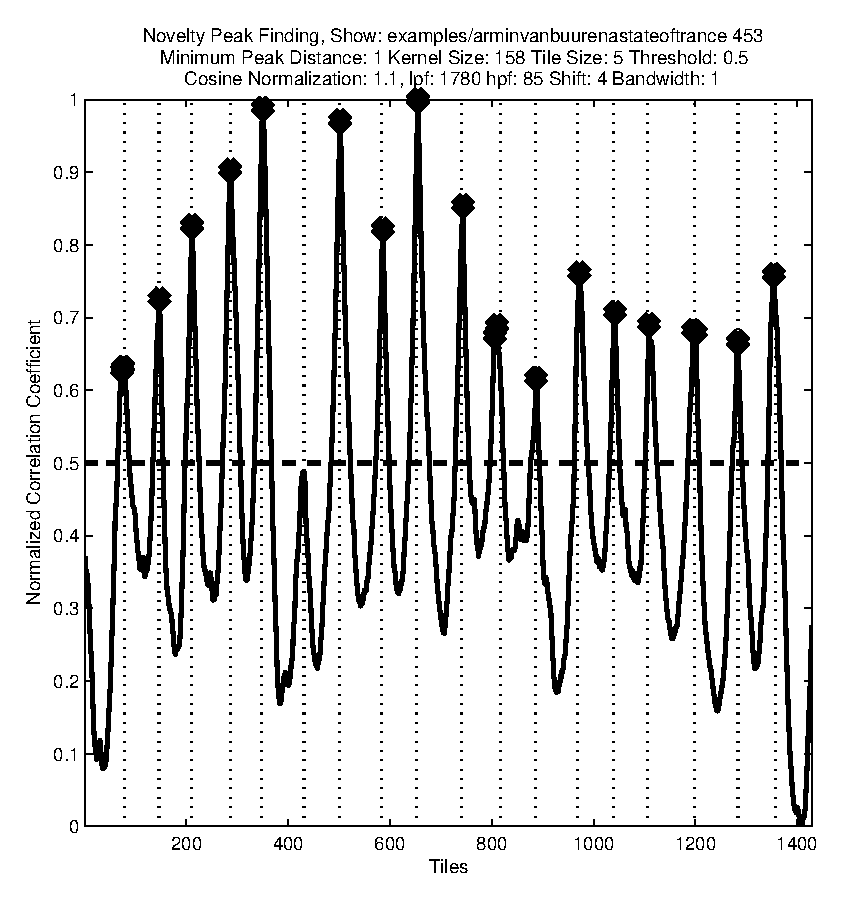
\includegraphics[width=0.45\textwidth]{images/novelty}
			
			
			\caption{Foote's novelty function for one of the radio shows in the corpus. The actual track indices are shown with dotted lines, and the predicted tracks are shown with the markers. Some of the parameters are drawn from our own method of constructing the self-similarity matrix (see Section~\ref{sec:feature-extraction})}
			
			\bigskip
			
			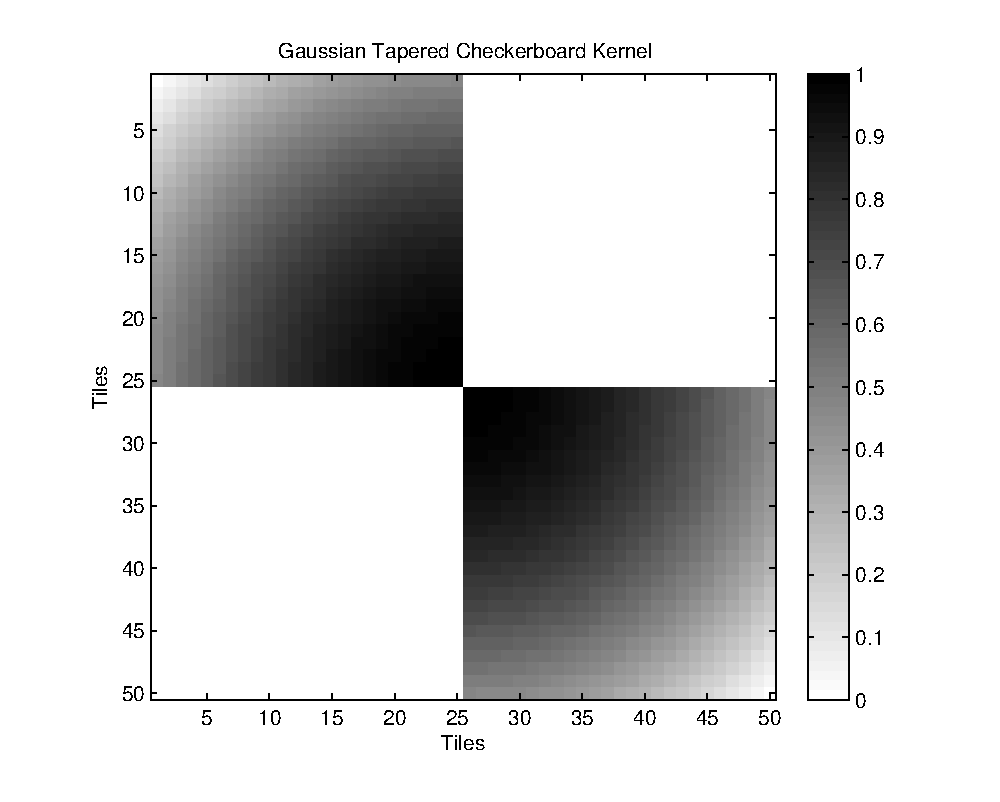
\includegraphics[width=0.5\textwidth]{images/checker}
			
				\caption{An example of Foote's Gaussian tapered checkerboard kernel, width 50.}
				
			
			\label{fig:novelty}
		\end{figure} 
	
	 Foote correlated a Gaussian tapered checkerboard kernel\citep{foote2003media} along the diagonal of a music self similarity (cosine) matrix to create a 1-dimensional novelty function that had the notion of self-similarity over a fixed time horizon. The kernel was `tapered' down to zero towards the edges by a multiplicative Gaussian kernel to reduce edge noise. Our approach in this paper can be thought of as having a \textit{soft} time horizon up to a fixed limit (Foote's work had a fixed kernel size). However, the drawback of our method is that we find a fixed number of tracks. Naturally; the width of the kernel strongly determines the shape of the resulting novelty function. Small kernels will highlight transient changes in the audio while larger kernels will operate over a larger time horizon.  
	
	Goodwin et al.\ used a dynamic program for segmentation \citep{goodwin2004dynamic}. Their approach was to perform linear discriminant analysis to project features into an a priori learned feature space. Afterwards, Goodwin formulated the problem into one of finding the globally minimum cost path through a state graph (the so called `cluster space trajectory') modelling local and transition costs between segments. Goodwin already demonstrated in \citep{goodwin2003audio} that novelty peaks often exist within segments, not only on the boundary of segments and took the approach of modelling all possible sequential transitions between all possible segments.
	
	A possible drawback to the approach by Goodwin and all other approaches in scene analysis segmentation that; is that they are somewhat local methods that focus on points-of-change rather than optimizing for the best possible results given a fixed number of segments to find. As Goodwin did not provide any results, we cannot conclude that a new distance function derived from learning a feature subspace improves segmentation accuracy. 
	
	Clustering algorithms do exist that find a fixed number of segments but we have the added constraint that these segments need to be homogeneous, contiguous and time-dependent. Radu \citep{radu} demonstrated a time-dependent modification of agglomerative (hierarchical) clustering for segmentation of music. A constraint was added such that during the algorithm clusters could only be merged if they were adjacent in time. Radu preprocessed the feature vectors to increase the homogeneity by averaging them over a sliding window of fixed size. Radu used a fixed number of clusters found as a stopping condition. The approach is model-free but by Radu's own admission lacks any form of regularization, possibly producing clusters that vary in size significantly. Radu modelled the segmentation as a binary classification problem (later also used by Badawy et al \citep{elaudio}) subject to threshold time horizons allowing standard performance metrics such as precision, recall and $F_1$ score to be used. 
	
	Stochastic model-based approaches to segmentation also have been devised. Levy et al use hidden Markov models in their approach to music segmentation in \citep{levy2008structural}, building on their previous work \citep{levy2006new, levy2006extraction}. Their HMM is based upon a generative Gaussian mixture model where each segment has a set of states, each generating a Gaussian distribution of feature vectors. A musical audio file can then be regarded as having an underlying sequence of states that generates the observed feature sequence. The HMM can then be trained with a priori knowledge. 
	
	Plotz et al also used a an HMM for segmenting DJ mixed music streams, further developing the concept of generic acoustic generators first described in \citep{batlle2002automatic}. Unfortunately Plotz only evaluated his method against a small corpus of unknown origin ($222$ minutes with $65$ song changes, compared to our $640$ hours with $6757$ song changes) and did not elaborate on the ground truth annotation methodology. 
	
	Badawy implemented a Foote (\citep{foote2003media}) inspired segmentation scheme to segment $61$ hours of recorded Montreux jazz festival concerts and compared to human captured ground truth meta-data. 
	
	In the coming sections we describe the corpus (Section~\ref{dataset}), human annotation accuracy (Section~\ref{human_acc}), how we handle data and deal with feature extraction and cost matrices (Section~\ref{sec:data-handling}), computing the best segmentation (Section~\ref{best_cost}), discussion of confidence intervals (Section~\ref{sec:confidence-intervals}), experiments (Section~\ref{sec:experiments}), and finally the conclusion (Section~\ref{conclusions}).
	
	\section{Corpus}\label{dataset}
	
	We have been supplied with several broadcasts from three popular radio shows. See Table~\ref{tab:corpus} for a description. The show genres are a mix of progressive trance, Uplifting Trance and Tech-Trance. 
	
	There are no silent gaps in the recordings. The shows come in $44100$ samples per second, $16$ bit stereo MP3 files sampled at $192$Kbs. We re-sampled these to $4000$Hz $16$ bit mono (left+right channel) WAV files to allow us to process them faster. We have used the \textit{Sound eXchange}\footnote{\url{http://sox.sourceforge.net}} program to do this. These shows are all $2$ hours long. The overall average track length is $5$ and a half minutes (slightly less for Magic Island (see Figure~\ref{fig:tracklengths})) and normally distributed.  There is a guest mix on the second half of each show. The guest mix DJs show off their skills with technically convoluted mixing, so it is fair to say that the boundary complexity increases during the guest mix and is at least not constant throughout the shows.
	
	An additional dataset of $36$ radio shows have been mixed by and annotated by Mikael Lindgren (the so called \texttt{lindmik} dataset). These shows are extremely useful because the DJ is the same person who created the ground truth time indices which should in theory reduce the amount of human confusion present in the annotation. Also there is less noise, for example voice-overs, guest mixes, radio show sounds, introductions etc. These shows also vary significantly in length from $1$ hour to nearly $5$ hours. There are $339$ shows in total.
	
	We believe this corpus is the largest of its kind used in the literature going on the comparative table of segmentation corpora listed by Peiszer et al in their literature review of audio segmentation \cite{peiszer2008automatic}. More recently Badawy et al \citep{elaudio} used a corpus of $61$ hours. The corpus we are using is longer than $640$ hours in length. 
	
\begin{table*}
	\centering
	\label{tab:corpus}
	\caption{Descriptive statistics about the corpus.}
	\bigskip
	\scalebox{0.7}{
		
		
	\begin{tabular}{llllllll}
	\textsc{Reference}        &	 \textsc{Name}                       &  \textsc{DJ}               & \textsc{Hours} & \textsc{Mean Tracks} & \textsc{Sum Tracks} & \textsc{Shows} & \textsc{Trk.~Length (S)} \\ \toprule
	\texttt{ASOT}    &	A State of Trance       &  Armin van Buuren & 198   & 20.6        & 2247       & 109   & 317.9           \\
	\texttt{MAGIC}   &	Magic Island            &  Roger Shah       & 198   & 17.3        & 1839       & 106   & 388.2           \\
	\texttt{TATW}    &	Trance Around The World &  Above \& Beyond  & 162   & 20.1        & 1771       & 88    & 329.8           \\
	\texttt{LINDMIK} &	On Cue                  &  Mikael Lindgren  & 83    & 25          & 900        & 36    & 331.1           \\ \toprule
	                 &	                        &                   & 641   & 20.7        & 6757       & 339   & 341.7
	\end{tabular}
}
\end{table*}

	\begin{figure}
		\centering
		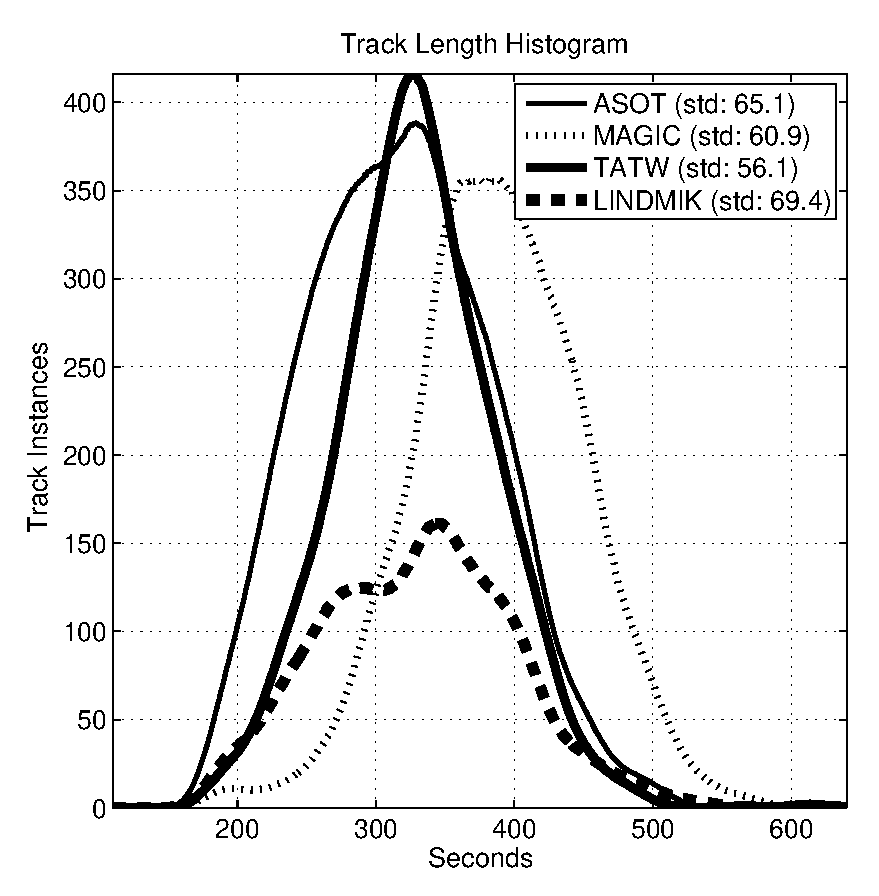
\includegraphics[width=0.45\textwidth]{images/trackhist}
		
		\caption{Track length histogram for all shows in the corpus.}
		
		\bigskip
		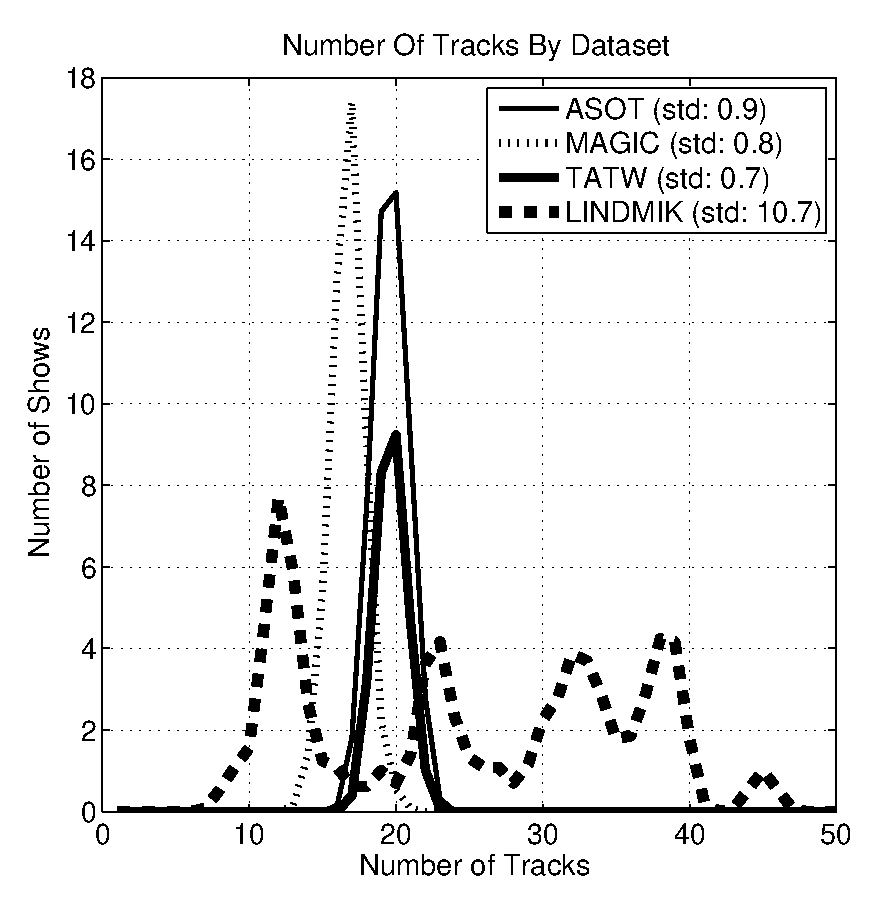
\includegraphics[width=0.45\textwidth]{images/numtracks}
		
		\caption{Number of tracks in each show for each dataset. The \texttt{lindmik} dataset is highly variable.}
		\label{fig:tracklengths}
	\end{figure} 
	
	There is already a large community of people interested in getting time annotations for DJ sets. \textit{CueNation}\footnote{\url{http://www.cuenation.com}} is an example of this. CueNation is a website allowing people to submit \textit{cue-sheets} for popular DJ mixes and radio shows. A cue-sheet is a text file containing time annotation meta-data (indices) for a media file.
	
	The three main radio shows in the corpus were hand captured by Denis Goncharov; a domain expert and one of the principal contributors to \textit{CueNation}. One of the significant problems with this task is that there is a small but apparent random confusion variable associated with the human captured indices in general (see Section~\ref{human_acc} for details) where 5\% of tracks get placed on a different bar. On some tracks, it is unclear where to place the optimal index on the macro scale and when analysing our results, we have noticed what we assume to be obvious human errors. Regrettably, there is no clear way of quantifying this. Many of the cue-sheet authors themselves reject the idea of automating the task, citing the poor precision of any such result (they often place indices on the exact MP3 frame). However this sentiment seems misplaced given that they frequently make mistakes or that it is a matter of opinion where to place the track and some consistent method may be preferential. A potential outcome of our method could be an assistance mechanism to help them with initial placements. Our results demonstrate that it is indeed possible to automate this task and that while there is some uncertainty attached to the optimal placement, it is still very predictable. Indeed on the majority of track indices the uncertainty is ostensibly small. 
	
	Denis Goncharov provided us with the following description of how he captures the indices. To quote from a personal email exchange with Denis:
	
	\begin{quote}
		Trance music is made in slices of $8$ bars. $1$ bar is $4$ beats. At $135$ beats per minute, $8$ bars is $(~60~/~135~)~\times~4 \times 8 = 14.8$ sec. Trance music tends to be around $130$-$135$ BPM. It is a matter of personal preference which point of the transition to call the index. My preference is to consider the index to be the point at which the second track becomes the focus of attention and the first track is sent to the background. Most of the time the index is the point at which the bass line ($400$Hz and lower) of the previous track is cut and the bass line of the second track is introduced. If the DJ decides to exchange the adjacent tracks gradually over the time instead of mixing them abruptly then it is up to the cue-sheet maker to listen further into the second track noting the musical qualities of both tracks and then go back and choose at which point the second track actually becomes the focus of attention.
	\end{quote}
	
	The most obvious and pervasive element in dance music is the percussion (the beats). We believe on balance that ignoring the percussive information is advantageous, because DJs use percussion primarily to blur boundaries between tracks.  We tried to capture percussive based features and found that the transitions between tracks and indeed groups of tracks appeared as stronger self-similar regions than the actual tracks. The percussive feature extractor transformed the autocorrelation of the audio samples in the time domain tiles, and compared the cosine of their absolute values. It was reasonably clear from that research that track boundaries are revealed with less uncertainty between instruments and harmonic content. However. We do not rule out looking at percussive features again the future because we are currently ignoring potentially useful information.
	
	Some DJs mix \textit{harmonically} (by matching instruments instead of percussion) but this preys on human hearing and perception. An algorithm capturing the harmonic information would still be able to distinguish two harmonically compatible tracks. 
	
	\section{Human Accuracy}\label{human_acc}
	
	We did some analysis on how accurate the humans themselves are at creating indices. In the absence of a perfect data set our analysis instead hinged on the amount to which the humans disagreed with each other aggregated over a large amount of historical data. Mikael Lindgren was kind enough to send us a dump of his cuesheet database to experiment with. As ASOT is such a popular show there were many independently captured cuesheets to compare against for all of the historical shows. We selected all the shows having at least $3$ distinct cuesheets (not copies or shifted/misaligned copies of each other)  and such that all the cuesheets had the same number of tracks. The first track was ignored (as it was always $0$ seconds). We ended up with $115$ shows with $3$ authors. $65$ shows with $4$ authors and $30$ shows with $5$ authors.  We generated a histogram of distances from the median time for each track, for each cuesheet and assumed values greater than $100$ seconds or less than $-100$ seconds were outliers. The standard deviation of the \textit{human disagreement} variable is $9.13$ seconds. See Figure~\ref{fig:human_muchconfuse} for an illustration. So at this stage it does not seem feasible for us to achieve a higher accuracy when we are evaluating against a method which is intrinsically error prone. An important caveat here is that ASOT turned out to be the most error-prone show to segment out of our corpus. The standard deviation of the bumps could be reduced if we normalized the times by the BPM of each transition. The \textit{bar-scale} confusion peaks centered around $\pm14.8$ seconds, and $\pm29.6$ seconds represented $5$ percent of the total annotations.
	
	\begin{figure}
		\centering
		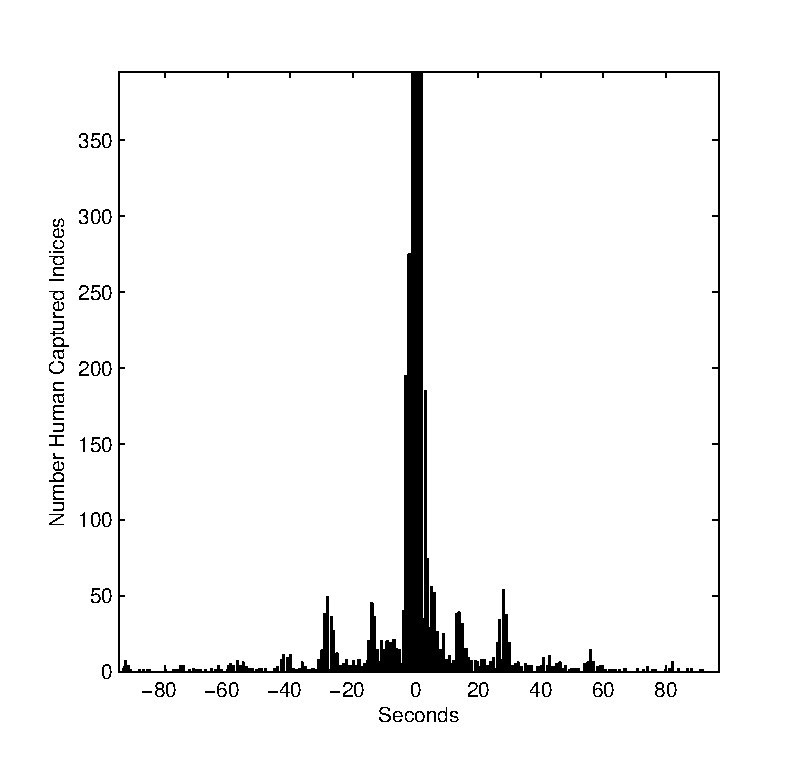
\includegraphics[width=0.45\textwidth]{images/human_confusion}
		
		\caption{Illustration of the `human disagreement' random variable (zoomed in at the bottom, the peak at $0$ seconds is $4708$ tracks), standard deviation $9.13$ seconds. Peaks are visible at intervals of $8$ bars ($14.8$ seconds) which corroborates the analysis from Denis Goncharov in Section~\ref{dataset}. The $4$ adjacent error clusters account for roughly 5 percent of the total number of tracks. The variance around the peaks represents the BPM variance in \texttt{asot}. }
		\label{fig:human_muchconfuse}
	\end{figure} 
	
	\section{Data Handling}\label{sec:data-handling}
	
	\subsection{Preprocessing}\label{proprocessing} % Fourier/xcorr
	
	The corpus had some outliers that may have slightly distorted the analysis of our method. Many of the tracks in the ground truth annotations for our corpus were actually introductions or voice-overs. Almost all of these outlier tracks were short in length. To ameliorate the situation we simply removed any tracks that were shorter than $180$ seconds (which are clearly not normal according to Figure~\ref{fig:tracklengths}). We also removed any end tracks that were shorter than $240$ seconds as very often the end tracks on a radio show contain peculiar elements (for example voice-overs, interviews, show-related `\textit{jingles}'). This required some manipulation of the cue-sheets and audio files. The undesirable segments of the audio files were chopped out, and the cue-sheets were re-flowed so that the time indices point to the correct location in the file. 
	
	The algorithm still performs similarly when removing just these indices and leaving the audio intact underneath, so it would not significantly affect any real-world implementation. 
	
	For those wishing to use this algorithm in practice with pre-recorded shows; the introductions at the start of the shows are often fixed length or at least predictable so error would be small on average.
	
	The \texttt{lindmik} dataset which was noise-free did not require any preprocessing whatsoever. 
	
	\subsection{Feature Extraction}\label{sec:feature-extraction}
	
	\subsubsection{Music}\label{feat_ex} % Fourier/xcorr
	
	We used \textit{Sound eXchange} (see Section~\ref{dataset}) to downsample the shows to $4000$Hz. We are not interested in frequencies above around and above $2000$Hz because instrument harmonics become less visible in the spectrum as the frequency increases. The Nyquist theorem \cite{nyquist1928certain} states that the highest representable frequency is half the sampling rate, so this explains our reason to use $4000$Hz. We will refer to the sample rate as $R$. Let $L$ be the length of the show in samples.
	
	Fourier analysis facilitates the representation of a time domain process as a set of integer oscillations of trigonometric functions. We transform the tiles into the frequency domain using the discrete Fourier transform
\[
F(x_k) = X_k = \sum_{n=0}^{N-1} x_n \cdot e^{-i 2 \pi \frac{k}{N} n}
\] which transforms a sequence of complex numbers $x_0,\ldots,x_N$ into another sequence of complex numbers $X_0,\ldots,X_N$ where $$e^{-i 2 \pi \frac{k}{N} n}$$ are points on the complex unit circle. Note that the fftw algorithm \cite{frigo2004fftw} that we used to perform this computation operates significantly faster when $N$ is a power of $2$ so we zero pad the input to the next power of $2$. We denote the tile width by $M$ in seconds (an algorithm parameter). Note that
\[
N = \frac{L}{M}
\] denotes the tile size in samples (length of show in samples over the tile size). Let 
\[
T = \left\lfloor\frac{L}{\tilde{M}}\right\rfloor
\] be the total number of tiles, and \[
\tilde{M}=\frac{L}{N}
\] the tile width in samples.
Because we are passing real values into the $F(x_k)$, the second half of the result is a rotational copy of the first half.
	
	Show samples are collated into a time series $Q_i^y$ ($T \times N$) of contiguous, non-overlapping, adjacent \emph{tiles} of equal size where $i=1,2,\ldots, T$. Samples at the end of the show that do not fill a complete tile get discarded. The affect of this is increasingly negligible with decreasing tile size. Since we zero-pad $N$ to the next power of two, this also decreases the affect.
	
	As we are not always interested in the entire range of the spectrum, we use $l$ to represent a low pass filter (in Hz) and $h$ the high pass filter (in Hz). So we will capture the range from $h$ to $l$ on the first half of the result of $F$. Let $\hat{h} = \lceil~h~\cdot~\frac{{N}}{R} ~\rceil+1$ be the position of $h$ in the spectrum, and $\hat l=~\lceil~l~\cdot~\frac{{N}}{R}~\rceil+1$ be the position of $l$ in the spectrum.
	
	Let $D_e^y$ ($T \times \hat{l}-\hat{h}+1$) denote the feature matrix.
	
	For each tile $\bar{i}=1,2,\ldots,T$ we assign 
\[
D_{\bar{i}}^{1,\ldots,\hat{l}-\hat{h}+1} = \left|~F(Q_{\bar{i}}^{1,\ldots,\tilde{M}})_{\hat{h},~\hat{h}+1,~\ldots,~\hat{l} }~\right|
\]
 selecting the part of the spectrum between the high and low pass filters $h$ and $f$.  We take the absolute values of the complex result of $F(x_k)$ (defined as its distance in the complex plane from the origin using the Pythagorean theorem).
	
	To accentuate instrument harmonics we perform convolution filtering on the feature vectors in $D$, using a Gaussian first derivative filter. This works like an edge detection/transient filter but also expands the width of the transients (instrument harmonics) to ensure that feature vectors from the same song appear similar because their harmonics are aligned on any distance measure (we use the cosines). This is an issue because of the extremely high frequency resolution from having such large inputs into $F(t_i)$. For example with a tile size of $10$ seconds and a sample rate of $4000$ we have a frequency resolution of $0.5 \cdot 10 \cdot 4000 = 20$KHz. 
	
	Typically a `short-time discrete Fourier transform' is used which has smaller sized inputs (windows) into $F(t_i)$ which are usually overlapping and are multiplied by a window function, attenuating the tails to reduce spectral leakage. Usually these window functions look similar to a Gaussian, for example;  
	\[
	\mathrm{Hann}_i = 0.5 - 0.5 \cos\frac{2\pi i}{n-1}{w(i)}
	\] where $n$ is the window size
	(see \cite{tzanetakis1999multifeature} for an example). The short-time Fourier transform is relevant when increased time precision is needed as there is a frequency-time resolution trade-off with respect of the input size to $F(t_i)$. This is not a concern in this particular application as our time resolution is never required to be better than $1$ second which would still produce adequate frequency resolution.
	
	The Gaussian first derivative filter is defined as 
	$$- \frac{2 \hat{\lambda}}{\upsilon^2}  e^{-\frac{\hat{\lambda}^2}{\upsilon^2}} $$ where 
	
	$$\hat{\lambda}=\left\{~-\lfloor 2\upsilon\rfloor,\lfloor-2\upsilon+1\rfloor,\ldots, \lfloor 2 \upsilon \rfloor~\right\},$$ and $$\upsilon = b  \frac{N}{R} .$$ $b$ is the bandwidth of the filter in Hz and this is a parameter of the algorithm. After the convolution filter is applied to each feature vector in $D$, we take the absolute values and normalize on the vector lengths.  
	
	Because the application domain is well defined in this setting, we can design features that look specifically for what we are interested in (musical instruments). Typically in the literature; algorithms use an amalgam of general purpose feature extractors. For example; spectral centroid, spectral moments, pitch, harmonicity \cite{tzanetakis1999framework}. We construct a dissimilarity matrix of cosines as is common in the literature for similar applications \cite{foote1999visualizing}. The cosines are computable easily because they are the the inner products of the respective features (the features have been normalized to unit length).
	
		\subsubsection{Self-Similarity Matrix}\label{sec:self-similarity}
	
	Let
	\[
	S_{ij} ~=~ 1-\langle D_{i}, D_{j}\rangle,
	\] define the dissimilarity matrix of cosines.
	
Then we apply some normalizing transformations. First we center $S$
around $0.5$ by raising each element to the power $2s$, where
$s=\frac{1}{T^2}\sum_{i,j=1}^TS_{ij}$. Since for $x\in [0,1]$ and
$y>0$ we have $x^y\le x$ if $y\ge 1$ and $x^y\ge x$ if $y\le 1$, the
transformation $S_{ij}\to S_{ij}^{2s}$ increases the values $S_{ij}$
whenever the mean value $s<0.5$ and decreases them whenever
$s>0.5$. Note that the transformation keeps the values $S_{ij}$ in the
interval $[0,1]$. We find this a convenient and gentle way to rescale
$S$.

Secondly we raise each value $S_{ij}$ to a power $\hat c \in
[0.5,1.5]$ and then rescale and translate them to $[0,1]$ using
$S_{i,j}\to 2S_{ij}-1$.  The parameter $\hat c$ is tuned so as to
achieve the right balance between negative \textit{incentives} and
positive \textit{disincentives} for meaningful track placement. We discovered in \citep{scarfe2013long}  that there was a pitfall of self-dissimilar regions within tracks negatively affecting the cost of placement. The distribution of values in $S$ after the transformations will have a
raised tail on left. This will become relevant when we discuss cost
matrices as some of them depend on the sign of the value in $S$.
	
	See Figure~\ref{fig:simmatrix} for an illustration of $S$ and Figure~\ref{fig:cosine_norm} for an illustration of the  normalization.
	
		\begin{figure}
			\centering
			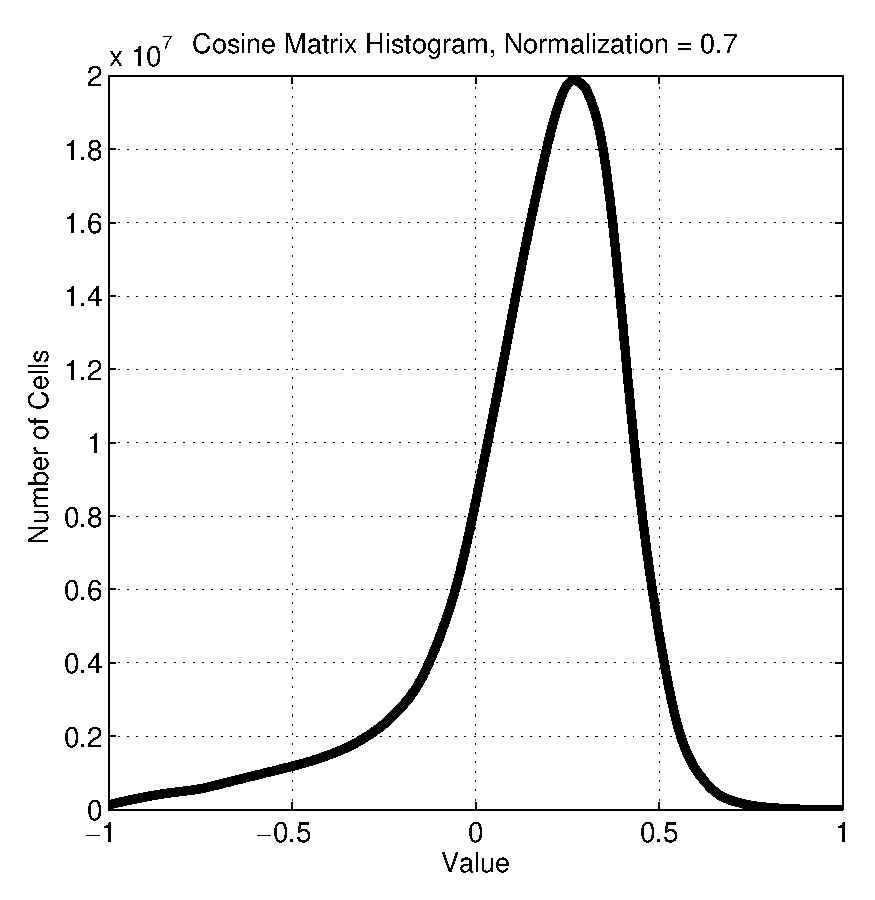
\includegraphics[width=0.35\textwidth]{images/cosine_histogram}
			
			\caption{Illustration of the effect of normalization parameter $\hat c=0.7$ on the values in $S$ on radio show \texttt{asot} $453$. The small raised section on the left correspond to the tracks down the diagonal.}
			\label{fig:cosine_norm}
		\end{figure} 
	
	\begin{figure*}[t]
		\centering
		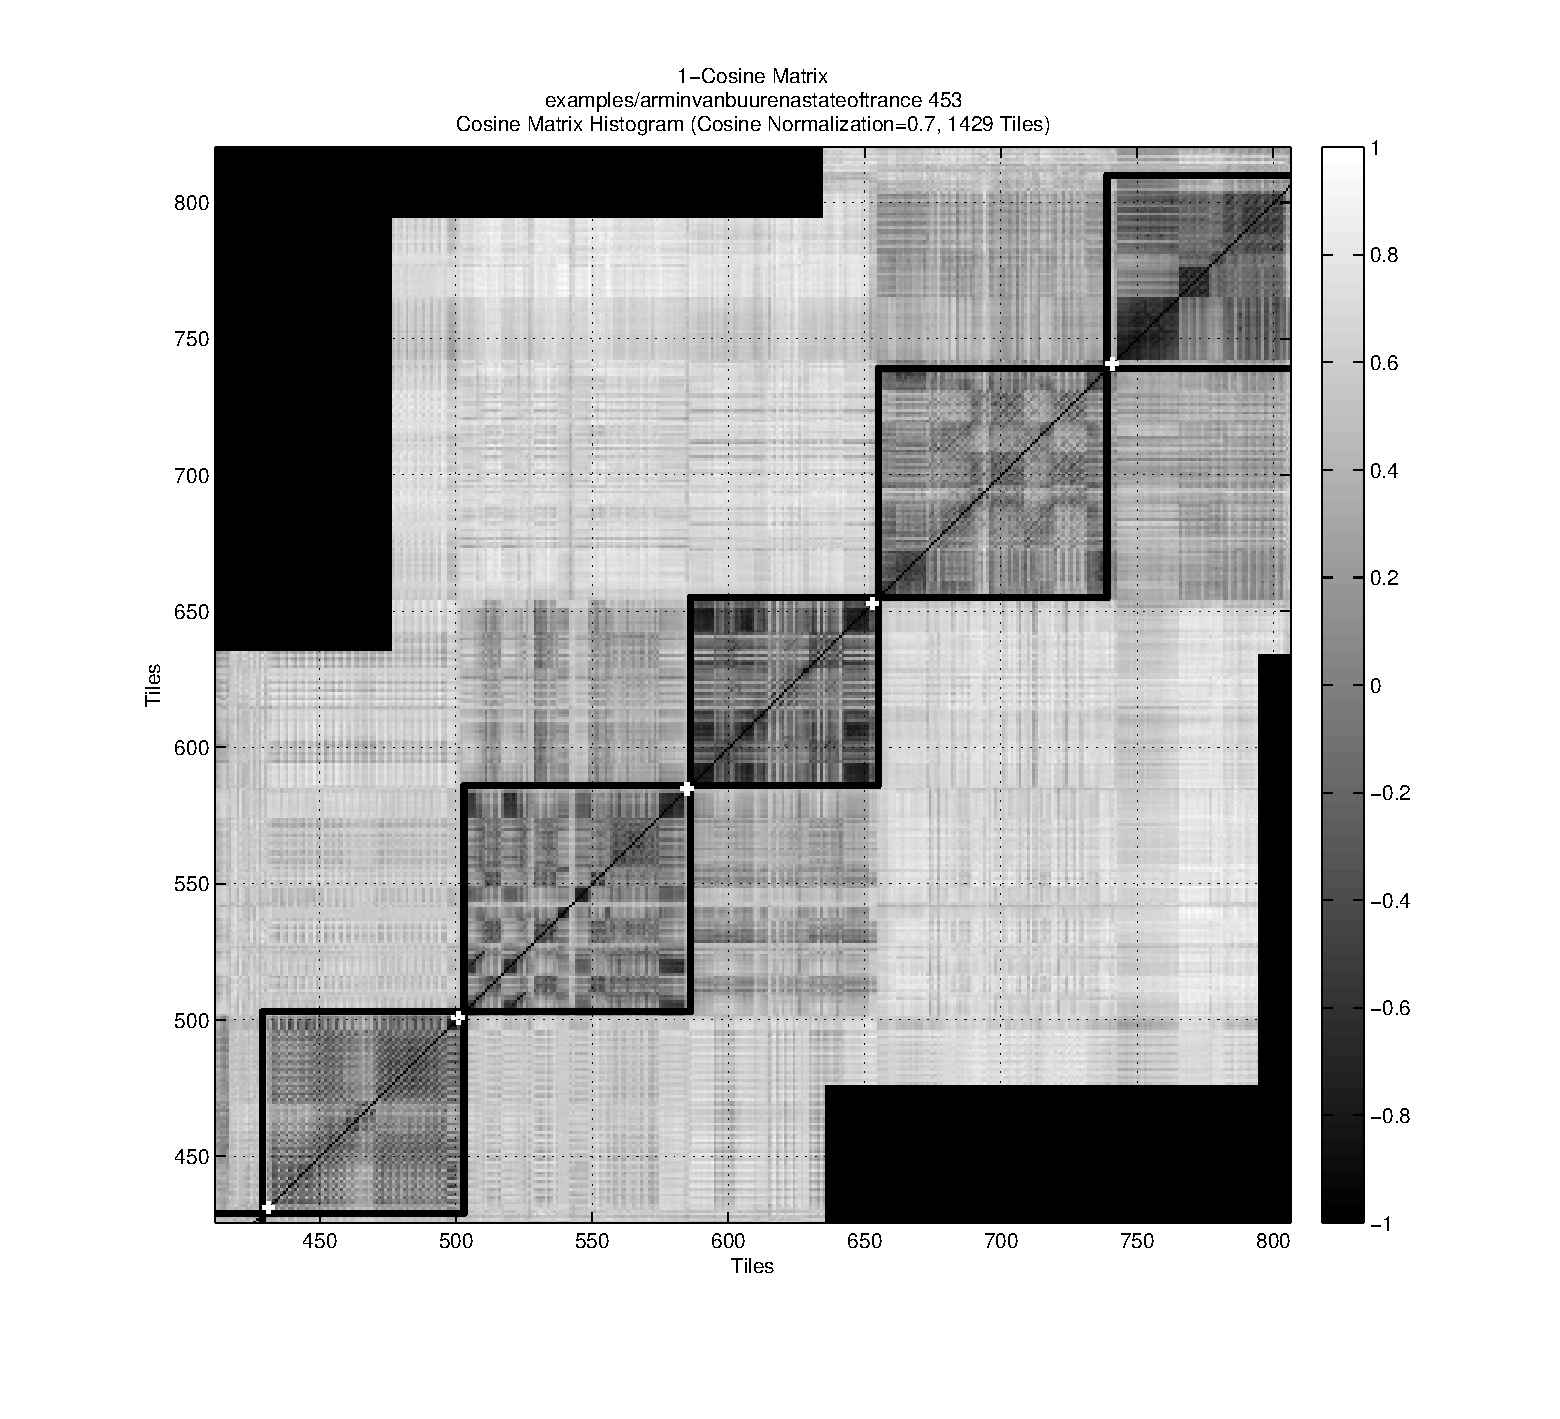
\includegraphics[width=1.08\textwidth]{images/cosines}
		\caption{An illustration of the similarity matrix $S$ (cosines) with the actual indices drawn on with black crosses, and our reconstructed annotations indicated with the dotted white lines. Note that to save time on the computation we do not calculate the entire matrix which is why there are some empty regions on the corners.}
		\label{fig:simmatrix}
	\end{figure*} 
	
	\subsubsection{Cost Matrices}\label{sec:cost-matrices}
	
	Let $w$ and $W$ denote the minimum and maximum track length in seconds, these are be parameters of the algorithm that will help improve the time complexity. 
	
We proceed to constructing a cost matrix $C(f,t)$ that describes the
cost of placing a track starting at $f$ and finishing at $t$ (and
having length $t-f+1$). After analysing the data set, we have created
$7$ cost matrices that exploit observed phenomena in $S$. We also
provide an additional cost matrix which is just a Gaussian random
function centred around the mean track length for all times which can
be used to regularise the other $7$ matrices or used on its own as a
comparator to a more naive method of placement.
	
	The cost matrices described in this section exploit themes such as contiguity, symmetry, evolution and change as well as simple summation of $S$ as was presented in our last paper \citep{scarfe2013long}. In our previous work $S$ was on the interval $[0,1]$ and the summation method could only consider disincentives. The new cost matrices have a parameter to shift the consideration of incentive versus disincentive and values on the interval $[-1,1]$.
	
	On the whole, a significant number of tile pairs within one track are similar to each other. Pairs of tiles that do not belong to the same track are expected to be dissimilar, most of the time. However, tracks have contiguous regions within them that are dissimilar to each other. Transitions between songs may appear as a self-similar region but usually also similar to each adjacent track to varying degrees.  
	
	\paragraph{Summation}\label{sec:summation}
	
	The most obvious strategy of all is to sum up all relevant tiles in $S$ for each candidate track from tile $f$ through tile $t$. We define $C(f,t)$, the cost of a candidate track from tile $f$ through tile $t$, to be the sum of the similarities between all pairs of tiles inside it
%it will be normalized at the end; it is easier to explain recursion without normalization

	\begin{dmath*}
	C(f,t, \omega, \bar S) =	\sum_{i,j=f}^{t} \frac{ \bar S }{ ( t - f + 1)^\omega }
	\end{dmath*}
where
	\begin{dmath*}
		\bar S \gets \hat S_{ij}(\Omega)=	{ \left\{
			\begin{array}{ll}
				 \Omega {S}_{ij},  & \text{~if~}{S}_{ij} > 0   \\
				 \left( 1-\Omega \right) {S}_{ij}, & \mbox{~otherwise~}\\
			\end{array}
			\right.} 
	\end{dmath*} 
for all $i,j \in {S}$. On this cost matrix, $\bar S$ and $\Omega {S}_{ij}$ are the same. Later we will use this summation function for modified $\bar S$. The quantity $\hat S$ is a modification of $S$ incorporating the \textit{incentive bias} parameter $\Omega$ which controls the balance of
positive and negative values. Direct computation using the definition
takes $O(TW^3)$ time. We can improve this to
$O(TW)$ by using the following recursion for the unnormalized quantity $\tilde C$ (assume that $f+1 \le t-1$, and note that the incentive bias parameter $\Omega$ has been temporarily removed for clarity):
	\begin{dmath*}
		\tilde C(f,t) = \tilde C(f+1,t) + \tilde C(f,t-1) - \tilde C(f+1,t-1) + \hat S_{ft} + \hat S_{tf}.
	\end{dmath*} 
The recursion implies that the cost of a track of length $L=t-f+1$ can
be calculated from the costs of shorter tracks using a constant number
of operations. The following picture provides an
illustration:
	
	\begin{center}
		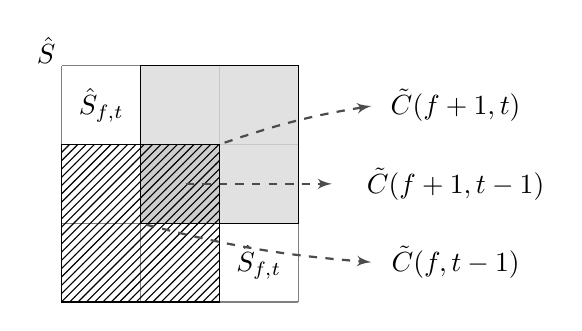
\begin{tikzpicture}
		\draw[step=1cm,color=gray] (0,0) grid (3,3);
		
		\draw[fill=gray!90, fill opacity=0.8] (1,1) -- (1,2) -- (2,2) -- (2,1) -- (1,1);
		
		\draw[fill=gray!30, fill opacity=0.8] (1,1) -- (1,3) -- (3,3) -- (3,1) -- (1,1);
		
	\draw [step=0.5cm, pattern=north east lines] (0,0) rectangle (2,2);
	
		
		\node[color=black] at (0.5,2.5) {$\hat S_{f,t}$};
		\node[color=black] at (2.5,0.5) {$\hat S_{f,t}$};
		
		\draw[color=black!70,->, >=latex', shorten >=2pt, shorten <=2pt, bend left=5, thick, dashed] 
		(2,2) to node[auto, swap] {}(4,2.5); 
		
		\draw[color=black!70,->, >=latex', shorten >=2pt, shorten <=2pt, bend right=5, thick, dashed] 
		(1,1) to node[auto, swap] {}(4,0.5); 
		
		\draw[color=black!70,->, >=latex', shorten >=2pt, shorten <=2pt, bend left=0, thick, dashed] 
		(1.5,1.5) to node[auto, swap] {}(3.5,1.5); 
		
		\node[color=black] at (-0.2,3.2) {$\hat S$};
		
		\draw[color=black] (0,0) -- (0,2) -- (2,2) -- (2,0) -- (0,0);
		\draw[color=black] (3,3) -- (1,3) -- (1,1) -- (3,1) -- (3,3);
		
		\node[color=black] at (5,0.5) {$\tilde{C}(f,t-1)$};
		\node[color=black] at (5,1.5) {$\tilde{C}(f+1,t-1)$};
		\node[color=black] at (5,2.5) {$\tilde{C}(f+1,t)$};
		
		
		\end{tikzpicture}.
	\end{center} 
	
	\bigskip

%	The final cost matrix is normalized by width and incentive bias
%\[
%C(f,t) \leftarrow \hat N_\Omega \left( \frac{ C(f,t) }{ t-f+1 } \right)
%\] for all $t,f \in \tilde C$.
	
	It is useful to scale cost matrices onto the interval $[0,1]$. Let normalization function
	
		\begin{dmath*}
			\hat N(x) + 1 = 2\frac{ x - \min_{ft}C(f,t) }{ \max_{ft} C(f,t) - \min_{ft} C(f,t)}.
		\end{dmath*}
	
	We proceed by applying this normalization; Let $C~\leftarrow~\hat N(C)$.
	
	See Figures~\ref{fig:cmsumib1} and \ref{fig:cmsumib2} for a image visualization of the summation cost matrix with different incentive biases.
	
	\paragraph{Symmetry}	
	
A common feature on dance music tracks is partial mirror-symmetry. We build a cost matrix to capture that.
	
Let $\Lambda(f,t,d)$ be the diagonal parallel to the minor diagonal
of $S$ and at the `distance' $d$ from it. We represent it as an ordered set
\begin{dmath*}
\Lambda(f,t,d)
 = \langle S_{f+d,f}, S_{f+d+1, f+1}, S_{f+d+2, f+2},\ldots, S_{t, t-d}\rangle.
	\end{dmath*} 
For each such diagonal in one triangle/half of $S$ we want to compare
each element against its mirror counterpart. For an ordered set
$\Lambda$ we define its cost as
\begin{dmath*}
\bar C(f,t,\bar \Omega)(\Lambda, \bar \omega)=\sum_{i=1}^{|\Lambda|} \frac{ \delta(\Lambda_i,\Lambda_{|\Lambda|-i+1},\bar \Omega)}{i^{\bar \omega}}
\end{dmath*}
where
\begin{dmath*}
\delta(p,q,\Omega) = 
\left\{\begin{array}{ll}
0,  & \text{if~}\sign( p ) \ne \sign( q ),\\
\Omega pq,   & \text{if~}  \sign(p) \ge 0 \text{~and~} \sign(q) \ge 0 ,  \\
(1-\Omega)pq,  & \text{if~} \sign(p) < 0 \text{~and~} \sign(q) < 0, \\
\end{array}\right.
\end{dmath*}
i.e., `symmetric' pairs that have the same sign make positive
contributions and pairs that have a different sign contribute $0$ to
the cost. We define the cost matrix as
\begin{dmath*}
\bar C(f,t,\bar \Omega, \bar \omega) = \sum_{d=1}^{t-f+1}\bar C(\Lambda(f,t,d,\bar \Omega), \bar \omega)
\end{dmath*}

Finally, let $\bar C~\leftarrow~\hat N(\bar C)$.

Clearly, one can reuse the cost for shorter intervals to calculate the
cost of longer ones, namely, $\bar C_{f+1,t-1}$ can be used to
calculate $\bar C_{ft}$ this saving computation time. We currently have an implementation on \textit{GitHub} (see Section~\ref{sec:materials}) with a time complexity of $O(TW^2)$

		\begin{center}
			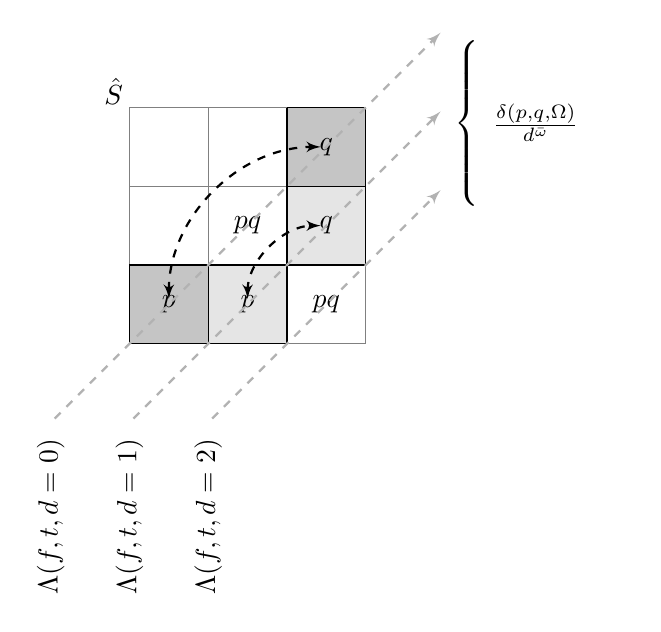
\begin{tikzpicture}
			\draw[step=1cm,color=gray] (0,0) grid (3,3);
			
			\draw[fill=gray!90, fill opacity=0.5] (0,0) -- (0,1) -- (1,1) -- (1,0) -- (0,0);
			\draw[fill=gray!90, fill opacity=0.5] (2,3) -- (3,3) -- (3,2) -- (2,2) -- (2,3);
			
			\draw[fill=gray!40, fill opacity=0.5] (1,0) -- (1,1) -- (2,1) -- (2,0) -- (1,0);
			\draw[fill=gray!40, fill opacity=0.5] (2,1) -- (2,2) -- (3,2) -- (3,1) -- (2,1);
			
			\node[color=black] at (-0.2,3.2) {$\hat S$};
			
			\node[color=black] at (0.5,0.5) {$p$};
			\node[color=black] at (2.5,2.5) {$q$};
				\node[color=black] at (1.5,0.5) {$p$};
				\node[color=black] at (2.5,1.5) {$q$};
			\node[color=black] at (2.5,0.5) {$pq$};
			\node[color=black] at (1.5,1.5) {$pq$};
			
			\node[color=black] at (-1,-2.2) { \begin{sideways}$\Lambda(f,t,d=0)$\end{sideways} };
			\node[color=black] at (0,-2.2) { \begin{sideways}$\Lambda(f,t,d=1)$\end{sideways} };
			\node[color=black] at (1,-2.2) { \begin{sideways}$\Lambda(f,t,d=2)$\end{sideways} };
				
			\node[color=black] at (5.2,2.8) { $ 
				\left\{ \begin{array}{ll}
				                   &  \\
				                   &  \\
				\frac{\delta(p,q,\Omega)}{ d^{\bar \omega} } &  \\
				                   &  \\
				                   &
			\end{array} \right. $  };
			
			\draw[<->, >=latex', shorten >=2pt, shorten <=2pt, bend left=45, thick, dashed] 
			(0.5,0.5) to node[auto, swap] {}(2.5,2.5); 
			
			\draw[<->, >=latex', shorten >=2pt, shorten <=2pt, bend left=45, thick, dashed] 
			(1.5,0.5) to node[auto, swap] {}(2.5,1.5); 
			
			\draw[color=gray!60,->, >=latex', shorten >=2pt, shorten <=2pt, bend left=0, thick, dashed] (-1,-1) to node[auto, swap] {}(4,4); 
			
			\draw[color=gray!60,->, >=latex', shorten >=2pt, shorten <=2pt, bend left=0, thick, dashed] (0,-1) to node[auto, swap] {}(4,3); 
			
			\draw[color=gray!60,->, >=latex', shorten >=2pt, shorten <=2pt, bend left=0, thick, dashed] (1,-1) to node[auto, swap] {}(4,2); 
			
			\end{tikzpicture}.
		\end{center}
	
	
	
%	Finally, the symmetry change matrix is defined where $\hat \delta$ is the same as the \textit{symmetry summation}, the width normalization is removed and the inner sum of the definition becomes the first order differences. For the sake of brevity we have omitted the dynamic programming formulations which run in $O(TW^2)$ time but they have been implemented in code and are available on-line (see Section~\ref{sec:materials}). This is also the case for all the following cost matrices.
	
\paragraph{Static Contiguity}\label{sec:static-contiguity}

Horizontal contiguous traces in $\hat S$ indicate that the track is
self-similar (negative values) or self-dissimilar (positive values)
due to repetition. If a given tile is the same as a set of contiguous
tiles following it, then there is some static contiguous region in the
show. The word \textit{static} denotes that the music is not evolving in
respect of time (which would instead create a diagonal trace in $S$).

We used the approach of modifying $S_{ij}$ in place (See Algorithm \ref{algo:contig}) so that we can use the fast summation algorithm described in Section \ref{sec:summation}. The algorithm takes the nth order differences (note that $\mathrm{diff}(x,2) = \mathrm{diff}(\mathrm{diff}(x))$ ) in two dimensions of $S_{ij}$, past and future. For simplicity our version of the diff function will return a matrix of equal size, zero-padded at the beginning. A brief introduction to the notation; $P(P>0)=5$ means to set all elements in $P_{ij}$ to $5$, and $\mathrm{diag}( \dot S, d ) \gets 5$ means set all elements in the $d$th diagonal of $\dot S_{ij}$ to 5.

Note that this algorithm introduces new parameters: $\dot p$ for the past nth order differences, $\dot f$ the future nth order differences, $\overleftarrow{\Omega}$ the past differences incentive bias, $\overrightarrow{\Omega} $ the future differences incentive bias. $\bar p$, how much contribution the past differences make, and $\bar f$ the future differences contribution. $\bar n$ is the normalization coefficient for this cost matrix. 



\begin{algorithm}
	\DontPrintSemicolon % Some LaTeX compilers require you to use \dontprintsemicolon instead
	$\dot s_{ij} = \mathrm{sign}(S_{ij})$ \\
	$P_{ij} \gets \mathrm{diff}( \hat S( \overleftarrow{\Omega} )^\intercal, \dot p )^\intercal$ \\
	$P_{ij} \gets \hat N( P )$ \\
	$ P(P < 0) \gets 1-|P(P < 0)|$ \\
	$ P(P > 0) \gets 1-|P(P > 0)|$ \\
	$ P_{ij} \gets  \bar p P_{ij}$, for all $i,j \in P$ \\

	$F_{ij} \gets \mathrm{diff}( \hat S( \overrightarrow{\Omega} ), \dot f )$ \\
	$F_{ij} \gets \hat N( P )$ \\
	$ F(F < 0) \gets 1-|F(F < 0)|$ \\
	$ F(F > 0) \gets 1-|F(F > 0)|$ \\
	$ F_{ij} \gets  \bar f F_{ij}$, for all $i,j \in F$ \\
	$\dot S \gets \dot s|P+F|$ \\
	$\dot S \gets \hat N(\dot S)$ \\
	
	$\mathrm{diag}( \dot S, d ) \gets \mathrm{diag}( \dot S, d ) d^{\bar n}$ for all $d \in \{1,2,\ldots,W\}$ \\
	$\dot S \gets \hat N(\dot S)$ \\

	\Return{$\dot S$}\;
	\caption{Construct \textit{contig-static} dissimilarity matrix by modifying $S_{ij}$ in-place.}
	\label{algo:contig}
\end{algorithm}
	
	
$\dot S$ is then transformed into a cost matrix $\vec{C}(f,t,\bar n,\dot s,\dot p,\dot f) = C(f,t, \omega, \dot S)$ using the summation function described in Section~\ref{sec:summation}.

	
\paragraph{Evolutionary Contiguity}

Any diagonal traces in $S$ that are parallel to the main diagonal are partial copies of the track in the future which evolve in respect of time. Evolutionary contiguity is a diagonal version of the static contiguity cost matrix described in Section~\ref{sec:static-contiguity}.



\begin{algorithm}
	\DontPrintSemicolon % Some LaTeX compilers require you to use \dontprintsemicolon instead

	
	\For{$d \gets 1$ \textbf{to} $W$} {
	
	$d \gets \mathrm{diag}( d )$ \\
	$s = \mathrm{sign}(d) $
	
	
	}
	
	\Return{$\dot S$}\;
	\caption{Construct \textit{contig-evolution} dissimilarity matrix by modifying $S_{ij}$ in-place.}
	\label{algo:contig}
\end{algorithm}


	\paragraph{Gaussian}
	Let \[
	G( \varpi, N )_{tw} = e^{ - \frac{1}{2} \frac{\varpi n}{ \frac{1}{2} W}^2  }
	\] for all $n=1,2,\ldots,W$ denote the Gaussian matrix cost function of $N\times W$. $G( \varpi, N )$ is time-independent and every row is the same. We will use this cost function for regularizing the others. It could also be used on its own for comparison against a `naive' cost matrix. Increasing values of $\varpi$ will tighten up the Gaussian. Note that we used values of $\varpi \in \{1,2,\ldots,5\}$
	
	\paragraph{Mixing Cost Functions}
	
	We mix cost matrices together by adding them. In our experiments we will have a parameter for each cost matrix $\in [0,1]$ to show its contribution to the mixture. The cost matrices will be multiplied by this number before being mixed. 
	
		\begin{figure}
			\centering
			\includegraphics[width=0.45\textwidth]{images/cmsumib0}
			\caption{Summation cost matrices for Magic Island episode 110 with an incentive bias $\Omega=1$ and therefore containing disincentives. }
			\label{fig:cmsumib1}
		\end{figure} 
		
		\begin{figure}
			\centering
			\includegraphics[width=0.45\textwidth]{images/cmsumib1}
			\caption{Summation cost matrices for Magic Island episode 110 with an incentive bias $\Omega=0$ and therefore containing incentives. }
			\label{fig:cmsumib2}
		\end{figure} 
		
		
	\paragraph{Solution Shift}
	
	We will also allow the estimated solution to be shifted in time by parameter $\varXi$ seconds $\in \{-5,-4,\ldots,5\}$.
	
	\section{Computing Best Segmentation}\label{best_cost}
	
	We obtain the cost of a full segmentation by summing the costs of its tracks. The goal is now to efficiently compute the segmentation of least cost.
	
	We want to reconstruct $m$ track boundaries ($m+1$ tracks).
	
	A sequence $\t = (t_1, \ldots, t_{m+1})$ is called an $m/T$-segmentation if and only if
	\[
	1 = t_1 < \ldots < t_m < t_{m+1} = T+1.
	\]
	$m$ is the number of tracks we are trying to find and is a parameter of the algorithm. We use the interpretation that track $i \in \{1, \ldots, m\}$ comprises times $\{t_i, \ldots, t_{i+1}-1\}$. Let $\segs^T_m$ be the set of all $m/T$-segmentations. Note that there are a very large number of possible segmentations 
	\begin{multline*}
		|\segs^T_m| ~=~ \binom{T-1}{m-1}
		= \frac{(T-1)!}{(m-1)!(T-m)!} =\\
		\frac{(T-1)(T-2)\cdots(T-m+1)}{(m-1)!} \ge \left( \frac{T}{m}\right)^{m-1}.
	\end{multline*} 
	For large values of $T$, considering all possible segmentations using brute force is infeasible. For example, a two hour long show with $25$ tracks would have more than 
	\[
	\left( \frac{60^2 \times 2}{25}\right)^{24}  \approx 1.06 \cdot 10^{59}
	\] possible segmentations. 
	
	We can reduce this number slightly by imposing upper and lower bounds on the song length.  Recall that $W$ is the upper bound (in seconds) of the song length, $w$ the lower bound (in seconds) and $m$ the number of tracks. With the track length restriction in place, the number of possible segmentations is still massive. A number now on the order of $10^{56}$ for a two hour show with $25$ tracks, $w=190$ and $W=60\cdot15$.
	
	Let $N(T,W,w,m)$ be the number of segmentations with time $T$ (in tiles),
	
	We can write the recursive relation $$N(T,W,w,m) = \sum N(t_m-1,W,w,m-1),$$ where the sum is taken over $t_m$ such that 
	\begin{align*}
		t_m &\le T-w+1 & t_m &\ge T-W+1\\
		t_m &\ge (m-1)w+1 & t_m &\le (m-1)W+1
	\end{align*}
	
	The first two inequalities mean that the length of the last track is within an acceptable boundary between $w$ and $W$. The last two inequalities mean that the lengths of the first $m-1$ tracks are within the same boundaries. 
	
	We calculated the value of $N(7000,60\cdot15,190,25)$ and got $5.20 \cdot 10^{56}$ which is still infeasible to compute with brute force.
	
	Our solution to this problem is to find a dynamic programming recursion.
	
	The loss of an $m/T$-segmentation $\t$ is 
	\[
	\loss(\t) 
	~=~
	\sum_{i=1}^m C(t_i, t_{i+1}-1)
	\]
	We want to compute
	\[
	\best^T_m ~=~ \min_{\t \in \segs^T_m} \loss(\t)
	\]
	To this end, we write the recurrence
	\begin{equation*}
		\best^t_1 ~=~ C(1, t) 
	\end{equation*}
	and for $i\ge2$
\begin{align*}
		\best^t_i ~=~& \min_{\t \in \segs^t_i} \loss(\t)  \\
		~=~& \min_{t_i} \min_{\t \in \segs^{t_i-1}_{i-1}} \loss(\t) + C(t_i, t)  \\
		~=~&  	\min_{t_i} C(t_i, t) + \min_{\t \in \segs^{t_i-1}_{i-1}} \loss(\t)  \\ 
		~=~& \min_{t_i} C(t_i, t) + \best^{t_i-1}_{i-1} \\
\end{align*}
	%On page 7: t_i should range from t-W to t-w. It is about the position of the /last/ song.
	
	In this formula $t_i$ ranges from $t-W$ to $t-w$. We have $T \times m$ values of $\best^T_m$ and calculating each takes at most $O(W)$ steps. The total time complexity is $O(TWm)$.
	
\section{Confidence Intervals}\label{sec:confidence-intervals}
	
It may be useful for some applications to build a framework to allow confidence intervals for our predicted indices. This may also be useful for meaningful comparison of cost matrices.
	
	\subsection{Posterior Marginal of Song Boundary}
	Fix a learning rate $\eta$, and fix $T$ and $m$. Let
	\[
	P(j,s) ~=~ 
	\frac{\displaystyle
		\sum_{\t \in \segs^T_m : t_j = s} e^{- \eta \loss(\t)}
	}{\displaystyle
	\sum_{\t \in \segs^T_m} e^{- \eta \loss(\t)}
}
\]
That is, $P(j,s)$ is the ``posterior probability'' that song $j$ starts at time $s$.

To compute $P(j,s)$, we need an extended notion of segmentation. We call $\t$ a $m/F: T$ segmentation if
\[
F = t_1 < \ldots < t_m < t_{m+1} = T+1.
\]
Let $\segs^{F : T}_m$ be the set of all $m/F-T$-segmentations. 
%
We have
\begin{multline*}
	\sum_{\t \in \segs^T_m : t_j = s} e^{- \eta \loss(\t)}
	~=~
	\sum_{\substack{\t \in \segs^{s-1}_{j-1},\\ 
			\t'\in \segs^{s : T}_{m-j+1}}} 
	e^{- \eta (\loss(\t) +\loss(\t'))}
	~=~ \\
	\left(\sum_{\t \in \segs^{s-1}_{j-1}} e^{- \eta \loss(\t)}\right)
	\left(\sum_{\t \in \segs^{s : T}_{m-j+1}} e^{- \eta \loss(\t)}\right)
\end{multline*}
%
which upon abbreviating
\begin{align*}
	\head^t_m & ~=~ \sum_{\t \in \segs^{t}_{m}} e^{- \eta \loss(\t)} &
	\tail^f_m & ~=~ \sum_{\t \in \segs^{f : T}_m} e^{- \eta \loss(\t)}
\end{align*}
means that we can write
\[
P(j,s) ~=~ \frac{\head^{s-1}_{j-1} \cdot \tail^{s}_{m-j+1}}{\head^T_m}
.
\]
So it suffices to compute $\head^{t}_{m}$ and $\tail^{t}_{m}$ for all relevant $t$ and $m$. We use
\begin{align*}
	\head^t_1 &~=~ e^{-\eta C(1,t)} &
	\tail^f_1 &~=~ e^{- \eta C(f, T-f+1)}
\end{align*}
and for $m\ge2$
\begin{align*}
	\head^t_m 
	&~=~ 
	\sum_{t_m} \sum_{\t \in \segs^{t_m-1}_{m-1}} e^{- \eta (\loss(\t) + C(t_m, t-t_m+1))} 
	\\
	&~=~ 
	\sum_{t_m} e^{-\eta C(t_m, t-t_m+1)} \sum_{\t \in \segs^{t_m-1}_{m-1}} e^{- \eta \loss(\t)}
	\\
	&~=~ 
	\sum_{t_m} e^{-\eta C(t_m, t-t_m+1)} \head^{t_m-1}_{m-1}
	\\
	\tail^f_m 
	&~=~ 
	\sum_{t_2} \sum_{\t \in \segs^{t_2 : T}_{m-1}} e^{- \eta (C(f, t_2-f)
		+ \loss(\t))}\\
	&~=~
	\sum_{t_2} e^{- \eta C(f, t_2-f)} \sum_{\t \in \segs^{t_2 : T}_{m-1}} e^{- \eta \loss(\t)}\\
	&~=~
	\sum_{t_2} e^{- \eta C(f, t_2-f)} \tail^{t_2}_{m-1}\\
\end{align*}

\begin{figure}
	\centering
	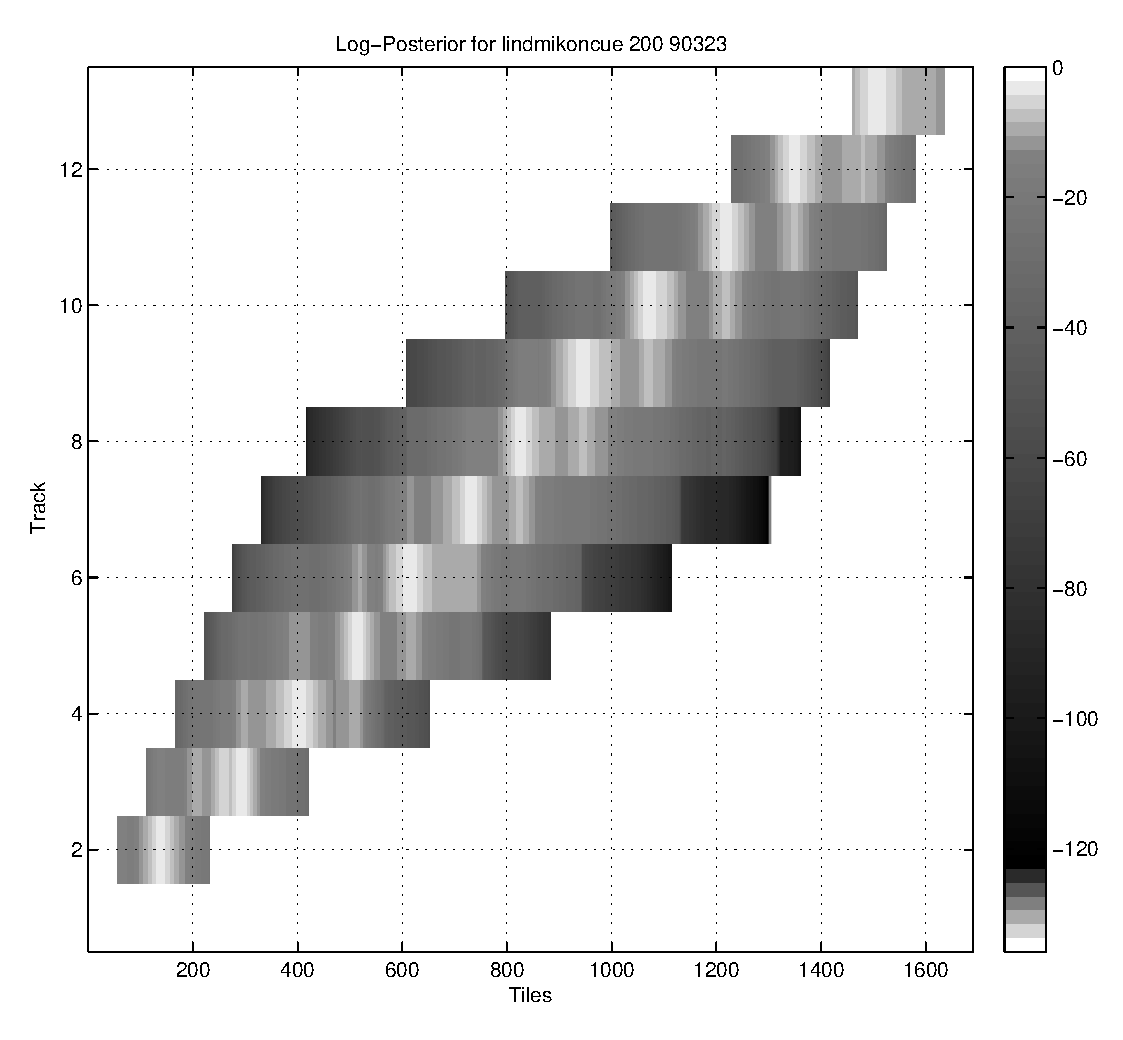
\includegraphics[width=0.5\textwidth]{images/posterior2}

	\bigskip

	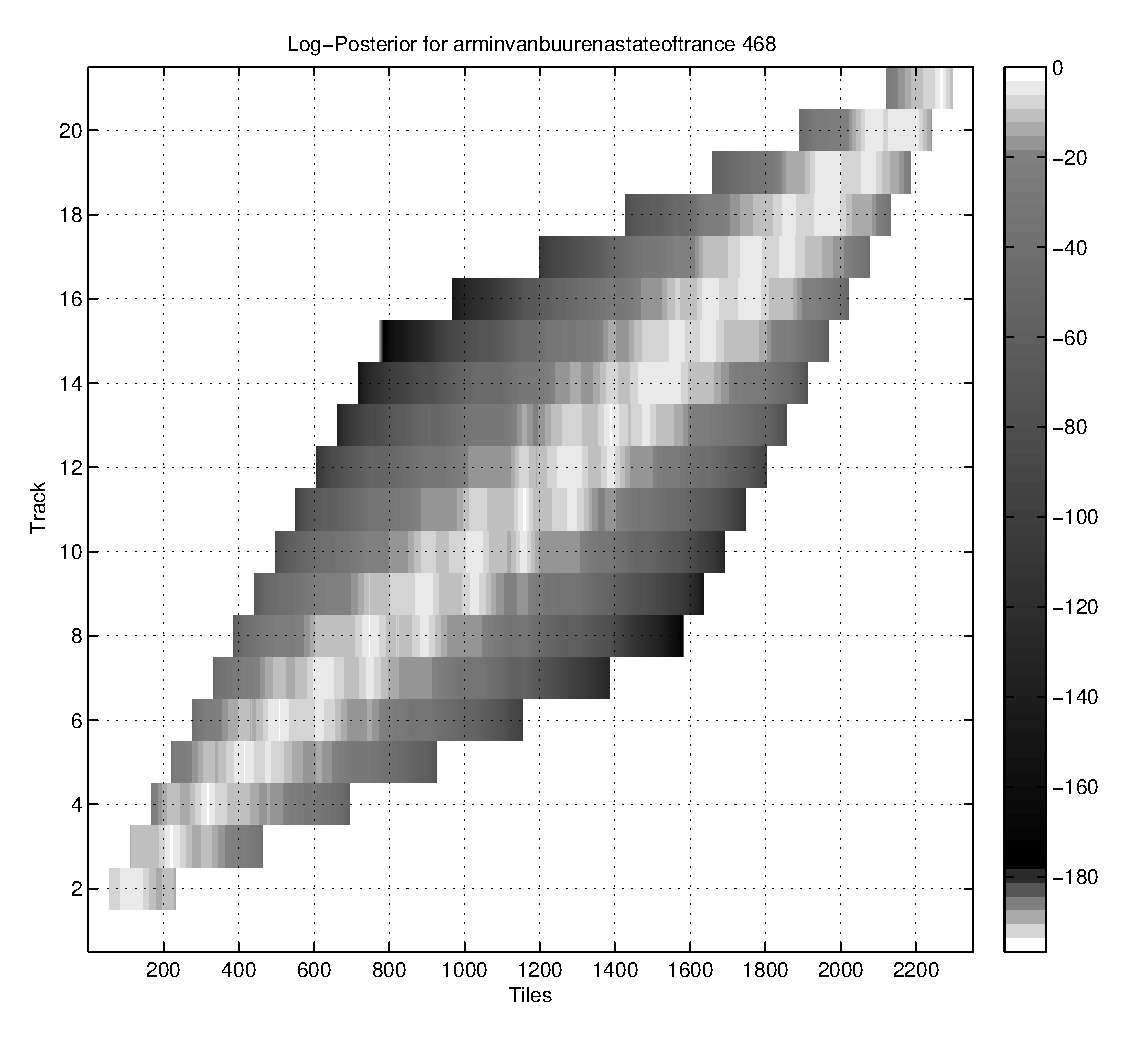
\includegraphics[width=0.5\textwidth]{images/posterior3}
	\caption{A visualization of $log(P(j,s))$ ($\eta=10$) for two of the shows in the training set. Ostensibly; uncertainty pertaining to the correct time and index (i.e. track number $2,3,4$) placement increases towards the middle of the shows.}
	\label{fig:posterior3}
\end{figure} 

See Figure~\ref{fig:posterior3} for an example of the posterior for a radio show. 

\subsection{Posterior Marginal of Song Position}
Fix a learning rate $\eta$, and fix $T$ and $m$. Let
\[
P(j,s,f) ~=~ 
\frac{\displaystyle
	\sum_{\t \in \segs^T_m : t_j = s \land t_{j+1}-1 = f} e^{- \eta \loss(\t)}
}{\displaystyle
\sum_{\t \in \segs^T_m} e^{- \eta \loss(\t)}
}
\]
That is, $P(j,s,f)$ is the ``posterior probability'' that song $j$ starts at time $s$ and finishes at time $f$.
%
In the same vein as the last section, we now get
\[
P(j,s,f) ~=~ \frac{\head^{s-1}_{j-1} \cdot e^{-\eta C(s, f-s+1)} \cdot \tail^{f+1}_{m-j}}{\head^T_m}.
\]


\subsection{Confidence Measures}

We can use the posterior marginal of song boundaries to give estimates of confidence on reconstructed indices where there are ambiguous options. The key scenarios where the algorithm is likely to make an error of judgement due to uncertainty are; getting the time wrong, the order wrong (for example, predicting the correct time in the wrong track index).

Note that the posterior marginal of song boundaries $P(j,s)$ contains values all in the interval $[0,1]$. The sum of all times for a fixed track index (every row) in $P(j,s)$ is $1$.

\subsubsection{Index (Order)}

To estimate the uncertainty of correct track alignment, we select the probability of all boundary placements for all track indices at the predicted best time. 

Let 
\[
\zeta_{ i} = P\left( j, \Pi\left(\best^T_m,j\right)  \right)
\] for all $j=1,2,\ldots,m$ where $\Pi(\best,i)$ will return the best time placement for index $i$ in the optimal segmentation $\best$.

Let the track index confidence measure 
\[
\Psi(\bar m)= 1- \frac{ \left(\tilde \zeta_{\bar m}\right) _2 }{ \left(\tilde \zeta_{\bar m}\right)_1 }
\] where $\tilde \zeta_{i}$ corresponds to $\zeta_{i}$ placed into in descending order of value. Note that $\Psi \in [0,1]$. The index confidence measure is a function of the ratio between the two largest values in $P(j,s)$ for all $j=1,2,\ldots,m$ and at the optimal time $s$ as estimated by the main algorithm. 




\subsubsection{Time}

The track time confidence is estimated by the ratio of the two highest peaks in $P(j,s)$ for all $s=1,2,\ldots,T$, for all $j=1,2,\ldots,m$.

Let 
\[
\xi(\bar m)= 1 - \frac{ \tilde \gamma\left( \bar m \right)  _2 }{ \tilde \gamma\left( \bar m \right)   _1 }
\] where \[
\gamma(j) = P(j,t)
\] for all $t \in 1,2,\ldots,T$ and $\tilde \gamma(j)$ are the peaks found in $\gamma(j)$ sorted in descending order. Note that $\xi \in [0,1]$



\section{Experiments}\label{sec:experiments}

\subsection{Training Set}\label{sec:training-set}

We selected $6$ shows at random (two of each show type)  to create a training set, which we will refer to as the \textit{GitHub training set}. See Table~\ref{table:githubset} to see the shows we selected.

\begin{table*}[t]
	
	\centering
	\caption{The shows randomly selected for inclusion in the \textit{GitHub training set}.}
	\label{table:githubset}
	\scalebox{0.8}{
	\begin{tabular}{llll}
		\toprule
		\#         & \textsc{Show Name}          & \textsc{Artist}  & \textsc{Date Broadcast} \\
		\toprule
		\textbf{1} & A State Of Trance 453       & Armin Van Buuren & April 2010              \\
		\textbf{2} & A State Of Trance 462       & Armin Van Buuren & June 2010               \\
		\textbf{3} & Magic Island 098            & Roger Shah       & March 2010              \\
		\textbf{4} & Magic Island 112            & Roger Shah       & July 2010               \\
		\textbf{5} & Trance Around The World 364 & Above \& Beyond  & March 2011              \\
		\textbf{6} & Trance Around The World 372 & Above \& Beyond  & May 2011 
		\\           
		\bottomrule   
	\end{tabular}
}
	
\end{table*}

\subsection{Number Of Tracks Known A Priori}\label{sec:apriori}

The primary goal of this research is to reconstruct optimal track boundaries when the number of tracks is known a priori. This experiment will pass the actual number of tracks as a parameter into the algorithm input variable $m$. The advantage of this is that the number of predicted tracks will equal the number of actual tracks so intuitive measures of predictive performance can be employed. 

\subsubsection{Evaluation}\label{eval_crit}

The inherent challenge with quantifying the performance of our approach is that if we misplace any tracks, it may have a cascade effect. For example if we place one track too many early on in a show, many of the subsequent tracks may be correctly detected but placed out of alignment. 

For the task of computing the best cost segmentation when the number of tracks are known a priori, we can use simple statistical descriptions of the track residuals $|P_{st}-A_{s't'}|$ where $P$ is the predicted track, $A$ the actual track, for show $s$ and track $t$ (for all $s$,$t$ and $s'$,$t'$ in the corpus). The mean average will give a good indication of the amount of misplacements (how robust the method is). The median of the residuals will indicate the actual track accuracy invariant to any catastrophic misplacements. The standard deviation of the residuals will indicate the spread of error. 

\subsubsection{Finding The Best Parameters}\label{sec:findingbestcostmatrix}

We used the GitHub (see Section \ref{sec:training-set}) training set to find robust algorithm parameters using a stochastic optimization (genetic algorithm) search. The genetic algorithm was selected because it allows integer constraints. We selected a population size of $50$, an elite count of $7$ and crossover fraction of $0.5$. The stopping limit for the algorithm was when the optimization objective function had stalled for $5$ generations. The \texttt{ga}\footnote{\url{http://www.mathworks.co.uk/help/gads/ga.html}} function from the MATLAB global optimization toolbox was used. 

We considered two objective functions; minimizing the mean absolute track error and secondly the median absolute track error (see Section~\ref{eval_crit}).

For each of these objective functions we devised $5$ conditional experiments involving a selection of cost matrices described in Section~\ref{sec:cost-matrices}; sum and Gaussian, symmetry and Gaussian, contiguity and Gaussian, evolution and Gaussian, and all cost matrices allowed. When cost matrices were not allowed to participate in an experiment, their contribution variable was fixed at $0$. Therefore; there are $10$ experiments defined. Robust parameters were found for each experiment using the genetic algorithm as described and the parameters found are listed in Table~\ref{tab:parameters}. An experiment number has been assigned to each configuration.

\subsubsection{Results}\label{sec:results}

Please see Tables~\ref{tab:mean-results} and~\ref{tab:median-results} for the results and Figure~\ref{fig:shifthistogram} for a histogram comparing track errors for experiments $1$ to $5$.

We notice that the \textit{contig-static}, \textit{evolution} and \textit{symmetry} cost matrices fail to perform well on their own. It was not really our intention to design these cost matrices to work well on their own but rather to augment the summation matrix. The Gaussian cost matrix then adds regularization. As reported in \cite{scarfe2013long}, the sum cost matrix performs robustly independently. When we consider the best combination of all cost matrices as defined by the results of the genetic algorithm (experiments $1$, $6$); the overall mean performance is improved substantially which means there are fewer catastrophic misplacements. 

\texttt{TATW} has the best overall performance (median 5 seconds on experiment $6$) and this is likely to indicate that it has an overall lower `complexity' of DJ-mixing.

We can conclude from these results that taking the best mixture of cost matrices significantly improves the robustness (mean-absolute of track errors) and spread (standard deviation of track errors) of the results. 

	\begin{figure}
		\centering
		
		\moveright 0.24cm \hbox{
		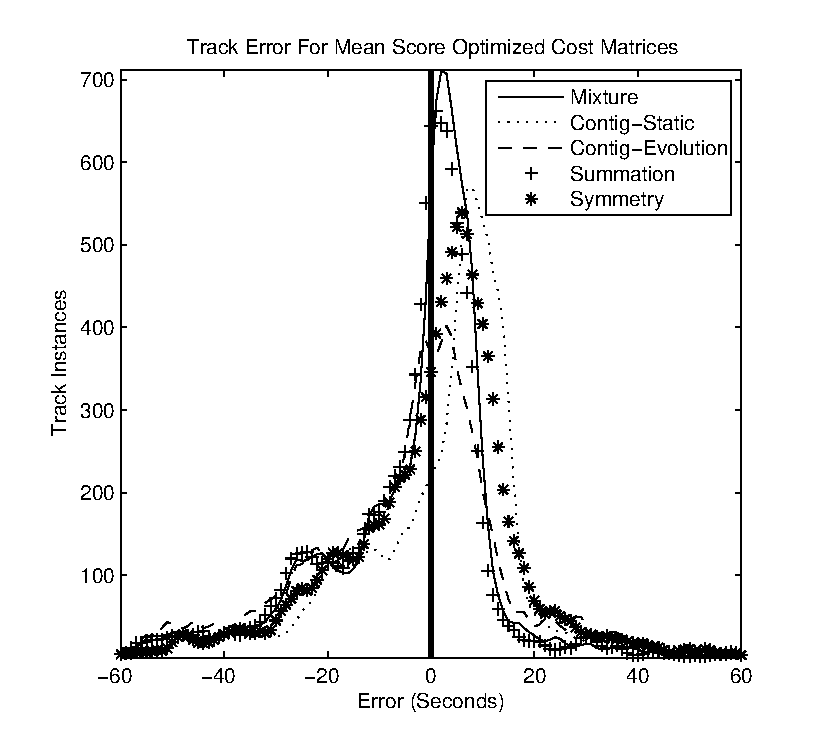
\includegraphics[width=0.46\textwidth]{images/shift_histogram}
		}
	
		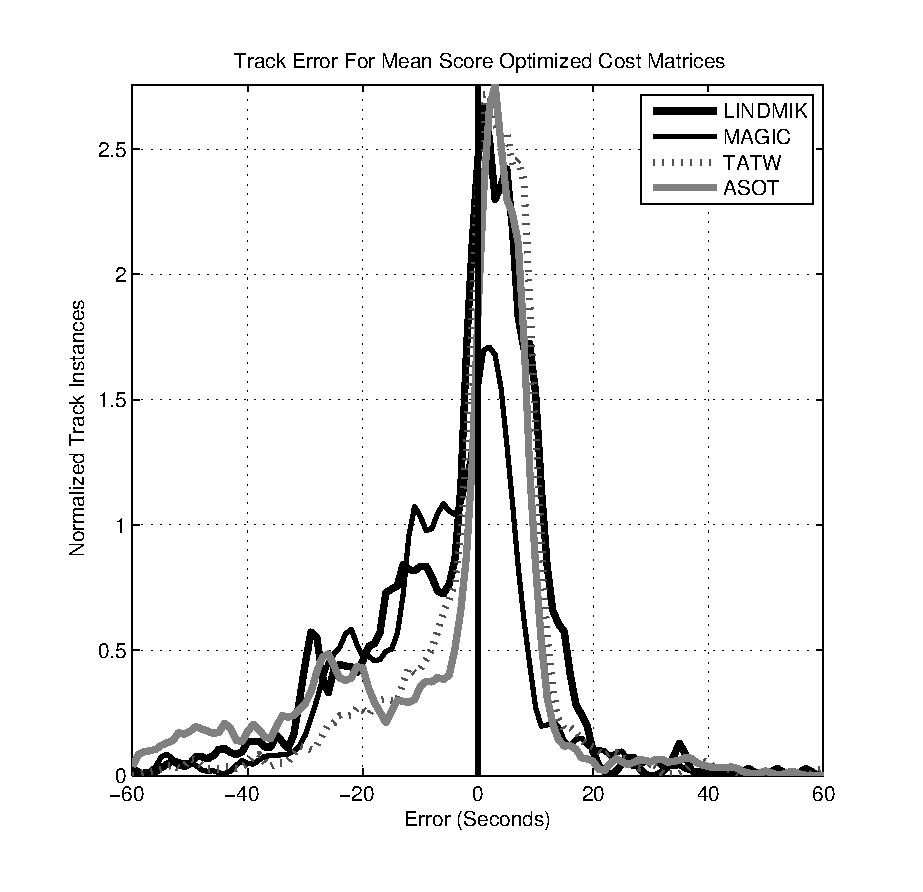
\includegraphics[width=0.5\textwidth]{images/residuals_byshow}
		
		
		
		\caption{Histogram of the residuals (errors) between reconstructed and human captured time indices per experiment (top) and with best mean-optimized mixture broken down by show (bottom). Apart from obvious noise there appears to be a tendency for the algorithm to place an index slightly earlier.    }
		\label{fig:shifthistogram}
	\end{figure} 

On \citep{scarfe2013long} we were effectively using a disincentive-only summation matrix, and found that normalizing costs on the square root of track length produced the best result. Something similar is happening here as the genetic algorithm has selected values less than $1$ on the sum normalization (experiments $4$,$9$) which would encourage placement of longer tracks. As opposed to \citep{scarfe2013long}, we no longer discard any shows from evaluation.

\begin{table*}[t]
	\centering
	\caption{These are the main results for all cost matrices with parameters optimized for the best mean absolute accuracy. The tuple $\langle a,b,c \rangle$ is used to indicate the results where $a$ is the median absolute error in seconds, $b$ the mean absolute error in seconds and $c$ the standard deviation in seconds (see Section~\ref{sec:results}). The experiment number is shown on the left.}
	\scalebox{0.9}{
	\begin{tabular}{lllllll}
		\toprule
		  &                        & \texttt{lindmik}                  & \texttt{magic}                   & \texttt{tatw}                    & \texttt{asot}                     & \texttt{all}                      \\ \midrule
		2 & \textsc{contig}        & $\langle 14,~70.3,~133.4 \rangle$ & $\langle 9,~18.6,~52.6 \rangle$  & $\langle 11,~34.6,~93.7 \rangle$ & $\langle 13,~58.5,~121.1 \rangle$ & $\langle 12,~42.9,~102.8 \rangle$ \\
		3 & \textsc{evolution}     & $\langle 14,~54.8,~110.2 \rangle$ & $\langle 12,~27.1,~58.4 \rangle$ & $\langle 9,~23.5,~54.6 \rangle$  & $\langle 15,~50.2,~101.8 \rangle$ & $\langle 12,~37.5,~83.3 \rangle$  \\
		4 & \textsc{sum}           & $\langle 8,~34.3,~81.1 \rangle$   & $\langle 8,~14,~34.3 \rangle$    & $\langle 6,~16.6,~50.26 \rangle$ & $\langle 8,~33.1,~77.3 \rangle$   & $\langle7,~23.7,~62.1 \rangle$    \\
		5 & \textsc{symmetry}      & $\langle 10,~20.4,~49.8 \rangle$  & $\langle 9,~16.6,~43.7 \rangle$  & $\langle 8,~11.7,~16.8 \rangle$  & $\langle 11,~26.2,~60.4 \rangle$  & $\langle 9,~19,~46.3 \rangle$     \\ \midrule
		1 & \textsc{all}           & $\langle 8,~19.5,~54.3 \rangle$   & $\langle 8,~16.9,~50.9 \rangle$  & $\langle 6,~8.9,~14.2 \rangle$   & $\langle 7,~24.3,~58.3 \rangle$   & $\langle 7,~17.6,~47.9 \rangle$   \\ \bottomrule
		  &
	\end{tabular}
}
	\label{tab:mean-results}
\end{table*}

\begin{table*}[t]
	\centering
	\caption{These are the main results for all cost matrices with parameters optimized for the best median absolute accuracy.}
	\scalebox{0.9}{
	\begin{tabular}{lllllll}
		\toprule
		  &                        & \texttt{lindmik}                  & \texttt{magic}                   & \texttt{tatw}                    & \texttt{asot}                     & \texttt{all shows}                \\ \midrule
		7 & \textsc{contig}        & $\langle 15,~96.3,~173.7 \rangle$ & $\langle 9,~28.4,~78.8 \rangle$  & $\langle 8,~51.5,~124.6 \rangle$ & $\langle 16,~78.1,~146.7 \rangle$ & $\langle 10,~60,~131.1 \rangle$   \\
		8 & \textsc{evolution}     & $\langle 20,~96.6,~149.8 \rangle$ & $\langle 13,~33.9,~69.8 \rangle$ & $\langle 8,~30.9,~76 \rangle$    & $\langle 18,~16.6,~114.8 \rangle$ & $\langle 12,~50.3,~104.5 \rangle$ \\
		9 & \textsc{sum}           & $\langle 8,~39.9,~95 \rangle$     & $\langle 8,~15.8,~42.5 \rangle$  & $\langle 6,~18.6,~59.7 \rangle$  & $\langle 7,~38.2,~90.2 \rangle$   & $\langle 7,~27.2,~73.0 \rangle$   \\
		10 & \textsc{symmetry}      & $\langle 12,~84.6,~161.8 \rangle$ & $\langle 9,~19.6,~51.5 \rangle$  & $\langle 9,~52.5,~127.9 \rangle$ & $\langle 18,~92.1,~171.2 \rangle$ & $\langle 11,~61,~135.5 \rangle$   \\ \midrule
		6 & \textsc{all}           & $\langle 6,~13.1,~28.7 \rangle$   & $\langle 9,~17.6,~44.7 \rangle$  & $\langle 5,~8.9,~15 \rangle$     & $\langle 6,~25.7,~62.4 \rangle$   & $\langle 6,~17.4,~44.8 \rangle$   \\ \bottomrule
	\end{tabular}
}
\label{tab:median-results}
\end{table*}

\begin{figure*}
	\begin{center}
		
		\begin{minipage}[t]{0.45\linewidth}
			\begin{center}
				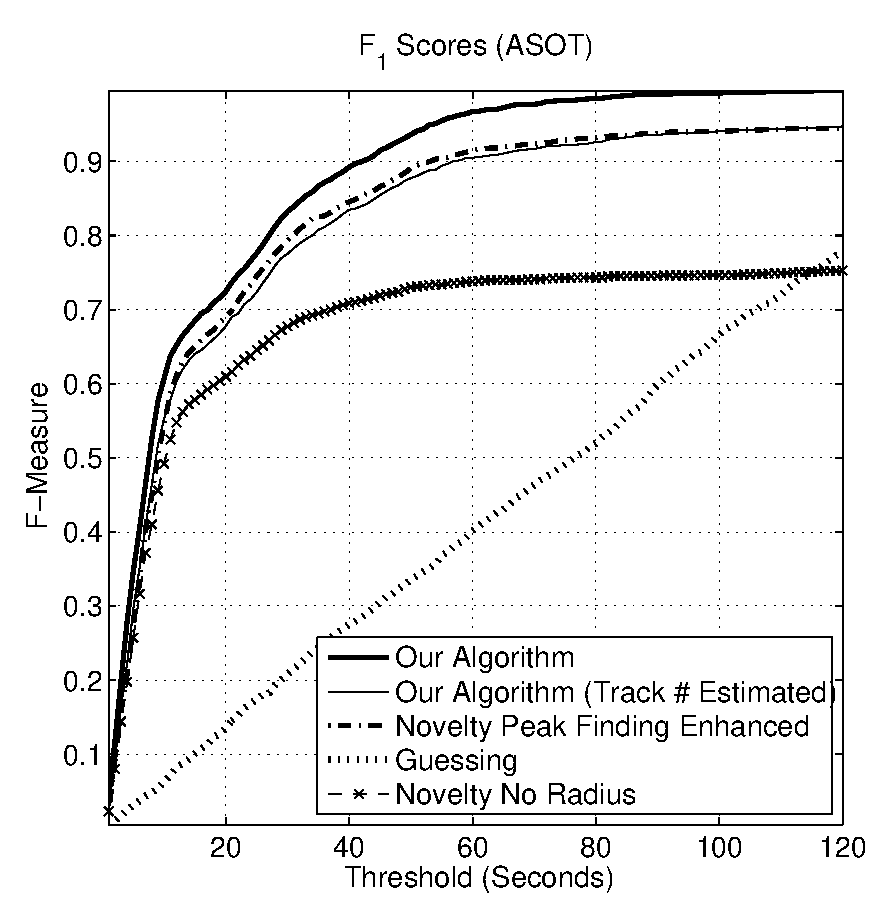
\includegraphics[scale=0.5]{images/fscores/fasot}
			\end{center}
		\end{minipage}
		\begin{minipage}[t]{0.45\linewidth}
			\begin{center}
				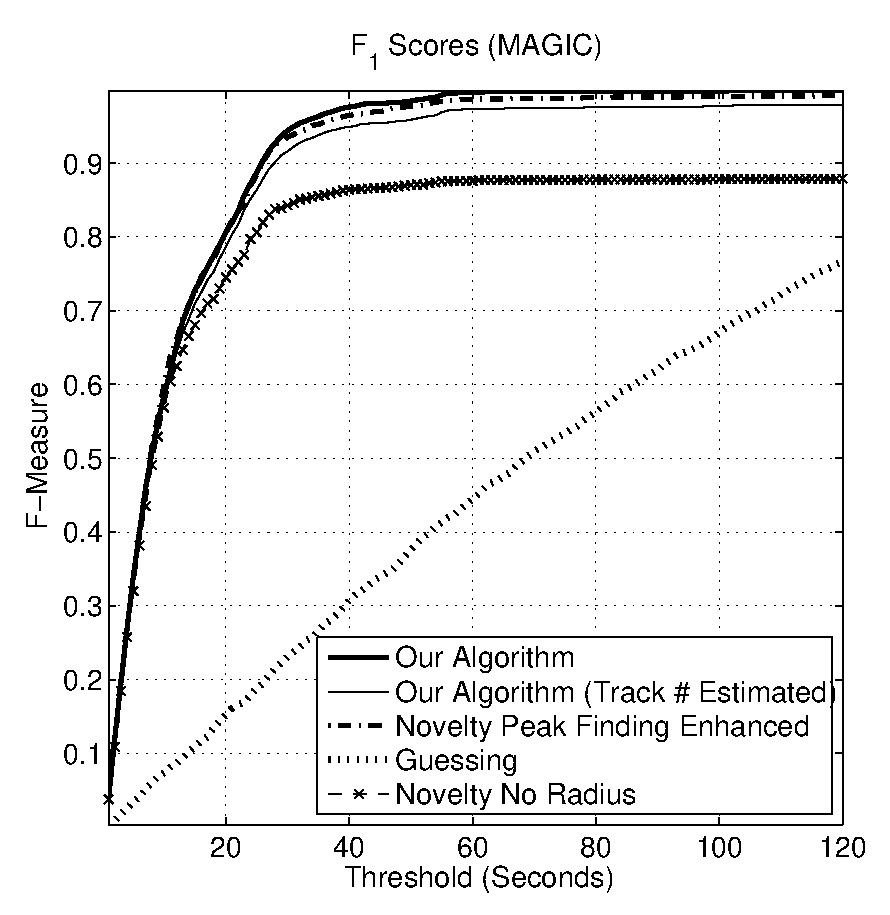
\includegraphics[scale=0.5]{images/fscores/magic}
			\end{center}
		\end{minipage}
		\bigskip
		
		\begin{minipage}[t]{0.45\linewidth}
			\begin{center}
				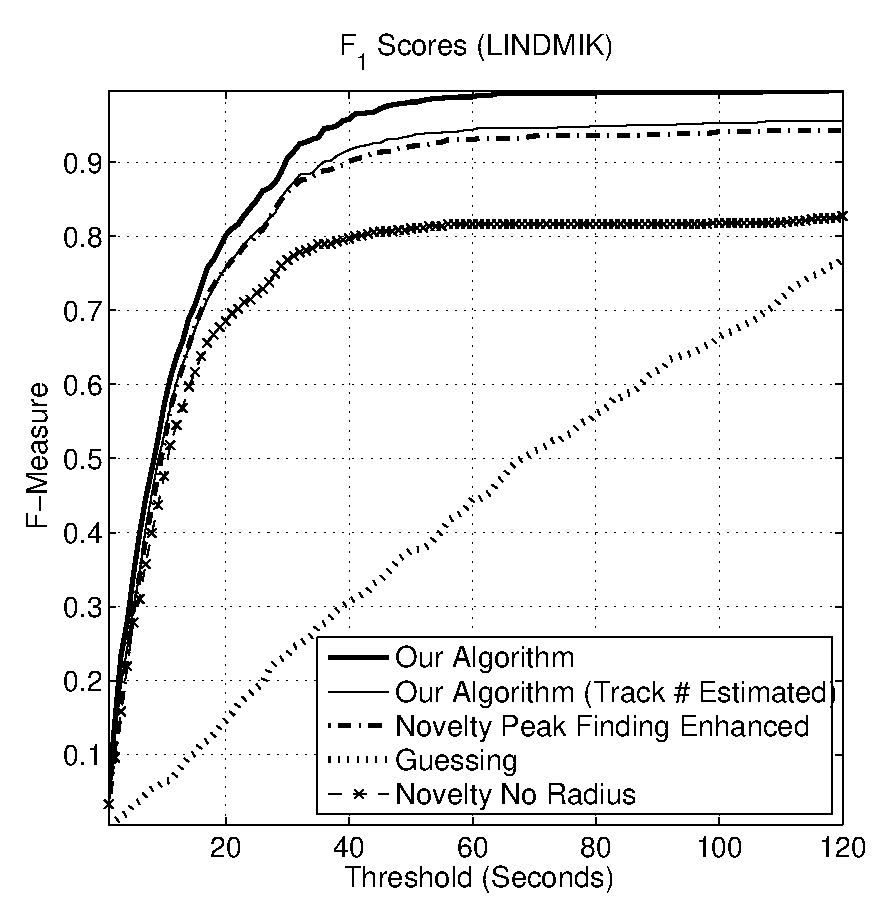
\includegraphics[scale=0.5]{images/fscores/lindmik}
			\end{center}
		\end{minipage}
		\begin{minipage}[t]{0.45\linewidth}
			\begin{center}
				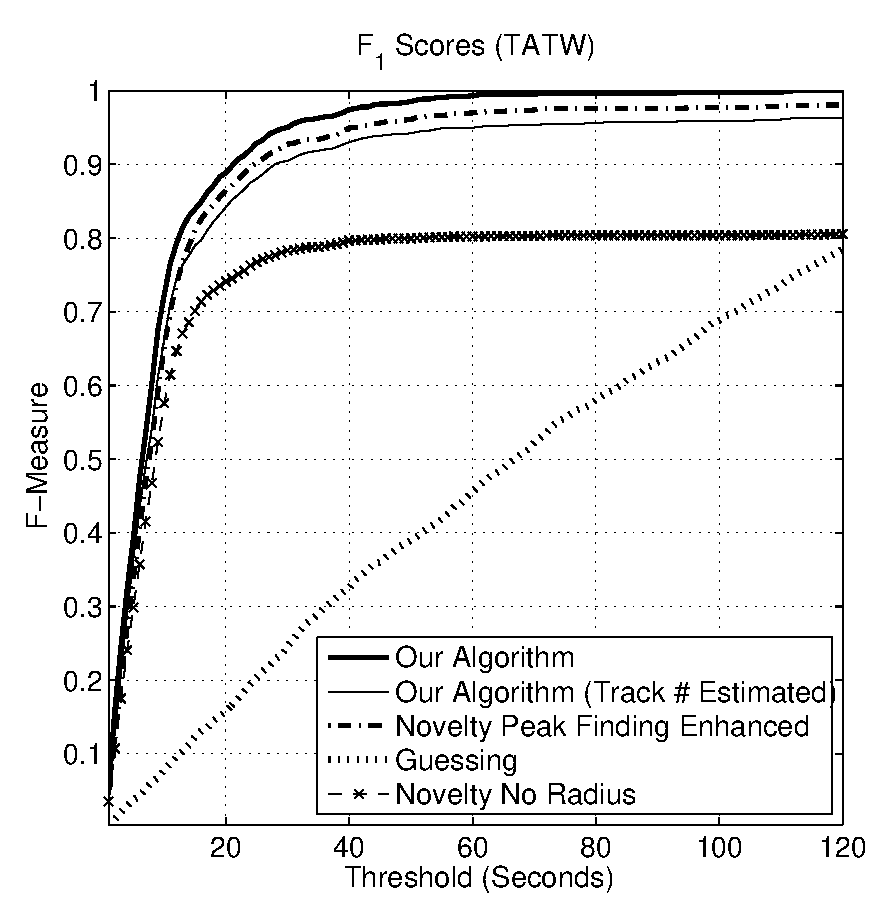
\includegraphics[scale=0.5]{images/fscores/tatw}
			\end{center}
		\end{minipage}
		
	\end{center}
	
	\caption{Comparison of the $F_1$ scores against time thresholds on the $4$ data sets. On the \texttt{lindmik} dataset where the number of tracks is highly unpredictable, our method combined with track estimation beats Foote's novelty method at higher thresholds.}
	\label{fig:fscores_breakdown}
		
\end{figure*}


\begin{figure}
	
		\begin{center}
			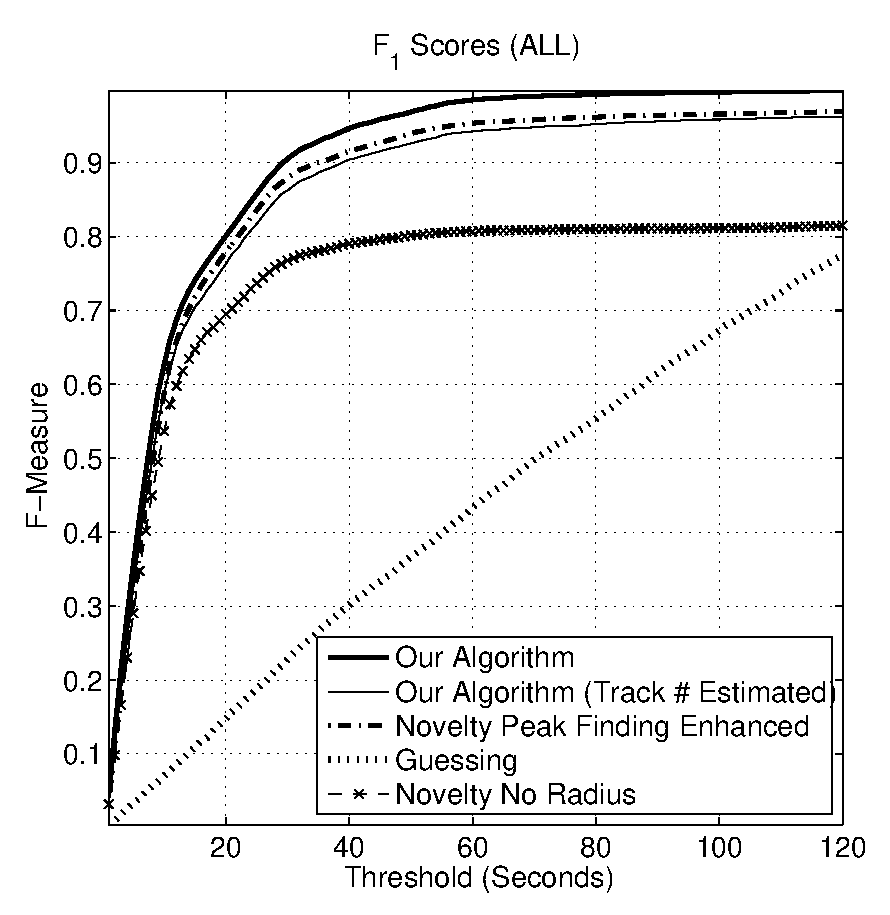
\includegraphics[scale=0.5]{images/fscores/fall}
		\end{center}

	\caption{Comparison between our algorithm and the Foote novelty peak finding approach on all of the datasets.}
	\label{fig:fscores_best}
	
\end{figure}

\subsubsection{Confidence Interval Analysis}

See Figure~\ref{fig:confidence_intervals} for illustrations of the time index confidence $\xi(\bar m)$, index placement confidence $\Psi(\bar m)$ and track error residuals averaged and shown as a function of progression through the shows. See Section~\ref{sec:confidence-intervals} for definitions. Because the number of tracks varies greatly, the confidence measures for all shows have been re-sampled into the set of indices $1,2,\ldots,15$. Thus it is possible to get an indication of aggregate confidence measures in relation to the progress of the show. 

We can conclude from these illustrations that the likelihood of placing the correct index statistically declines towards the middle of the shows. Perhaps this means that the summation matrix would have performed increasingly poorly as show lengths got longer. But mixing the cost matrices together in the optimal way (as dictated by the results of the evolutionary algorithm) apparently removes this tendency to a large extent. 

A low index confidence would increase the probability of a \textit{catastrophic misplacement} causing a significant deterioration on the overall mean performance metric. So these illustrations give us some insight on why mixing the cost matrices together significantly affected the overall mean evaluation metric as described in Section~\ref{sec:results}.    

Mixing the cost matrices had little effect on the time placement of indices. 

\begin{figure}
	
	\centering
	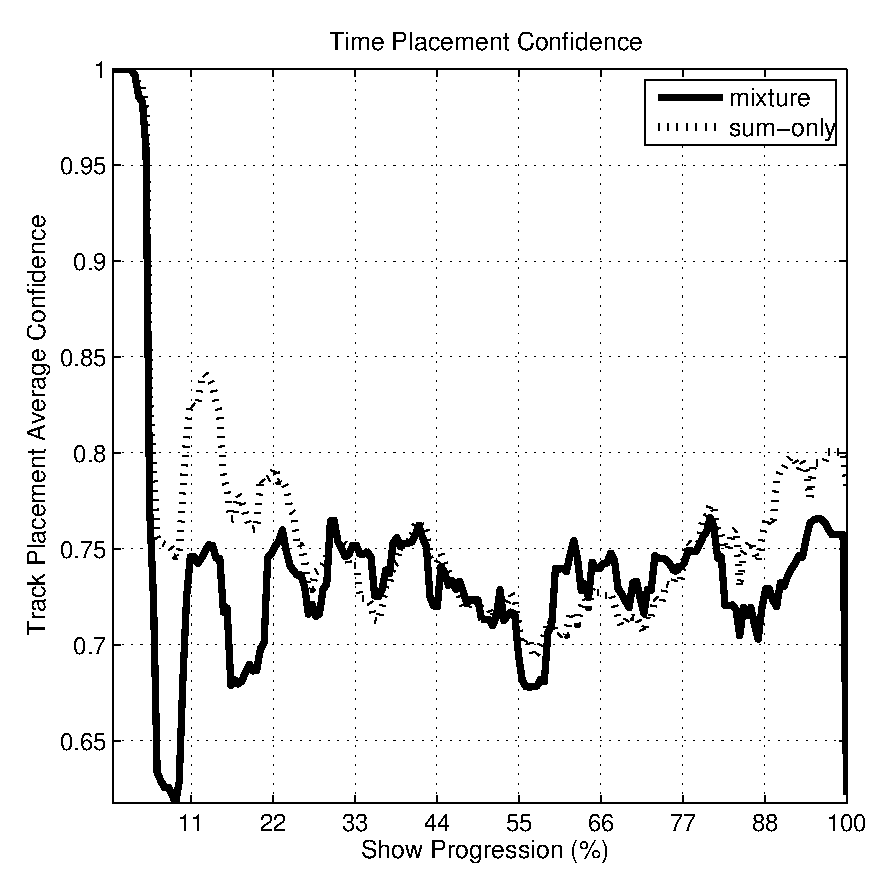
\includegraphics[scale=0.4]{images/conf/timeplacementconfidence}
	\bigskip
	
	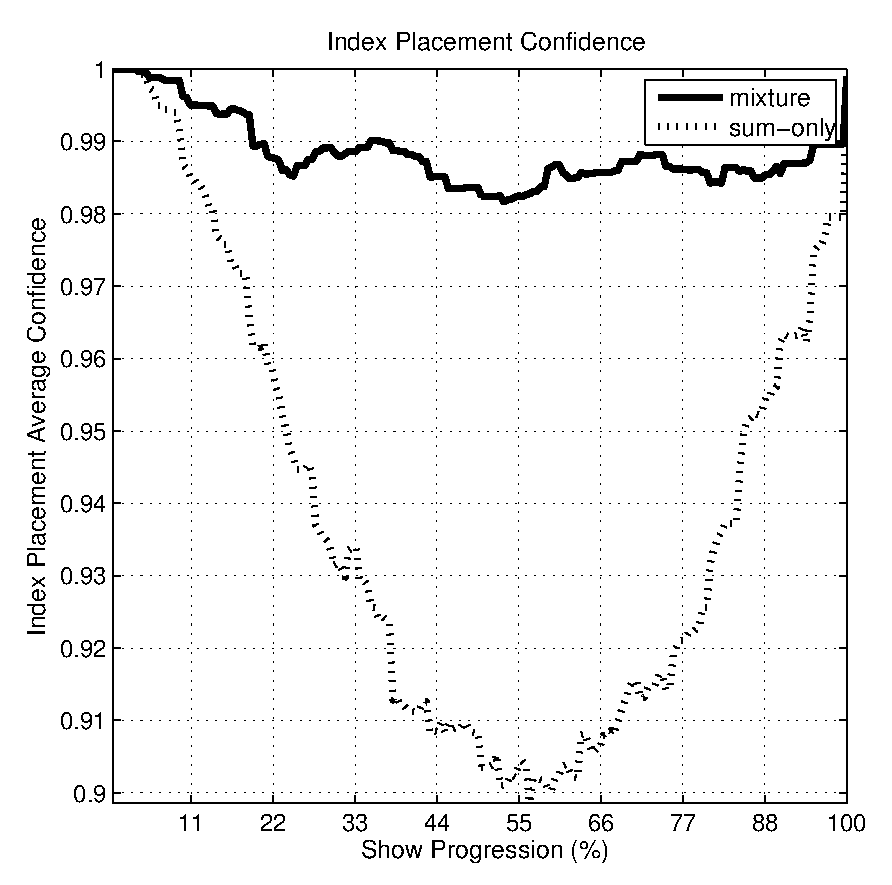
\includegraphics[scale=0.4]{images/conf/indexplacementconfidence}
	\bigskip
	
	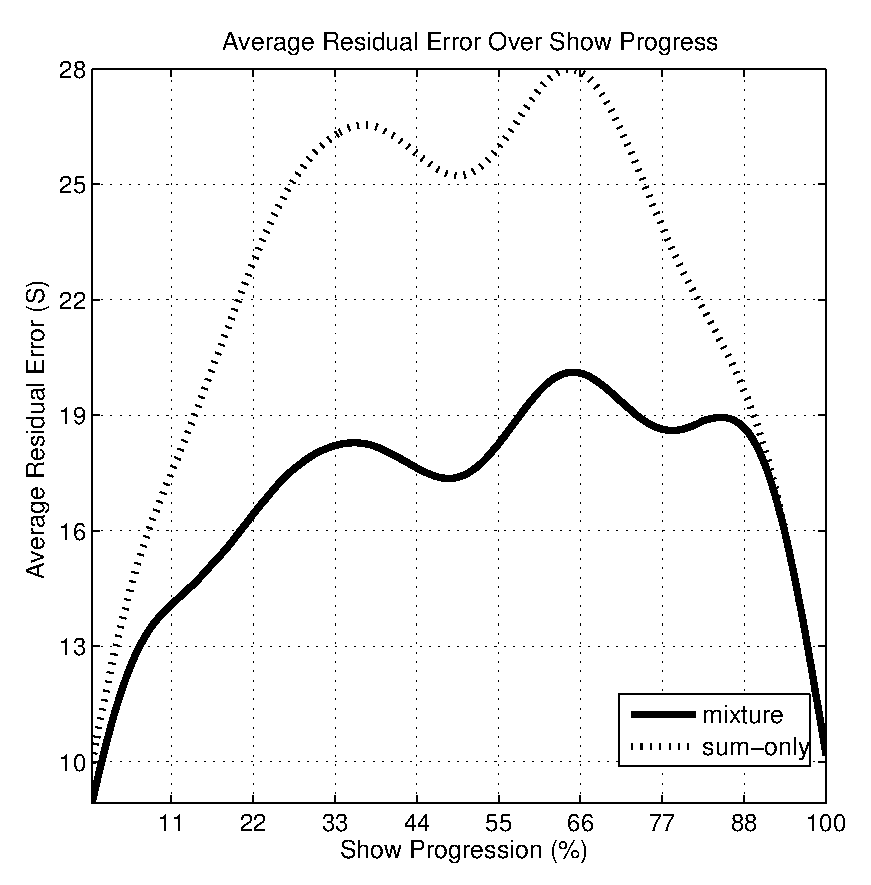
\includegraphics[scale=0.4]{images/conf/residualsagainstprogress}
	
	\caption{Confidence intervals and error residuals averaged over show progression.}
	\label{fig:confidence_intervals}
	
\end{figure}


% GENETIC ALGORITHM DESCRIPTION
\subsection{Number Of Tracks Not Known A Priori}\label{sec:trackcount}

The main goal of our research is providing the best possible time dependent contiguous segmentation given a fixed number of tracks $m$, rather than estimating $m$. This problem has not been addressed before to our knowledge; namely that the number of segments is known a priori but segmentation itself is not. However, the number of tracks could be estimated in a naive sense because the variable of track lengths is Gaussian (see Figure~\ref{fig:tracklengths}). 


We propose the following method of adapting our framework to estimate the number of contiguous segments in a data stream. For every possible candidate number of tracks $\vartriangle$, compute the cost of fitting $\vartriangle$ tracks using the algorithm described in Section~\ref{best_cost} and normalize it by $\vartriangle$ and take the solution $n$ on the saddle point where the normalized quantity achieves the minimum (see Figure~\ref{fig:github_trackestimation} for an illustration). We ran the same genetic algorithm as described in Section~\ref{sec:findingbestcostmatrix} to find the best set of parameters for this task. This is referred to as experiment $11$ in Table~\ref{tab:parameters}.

For comparison; we have implemented Footes method of segmentation \citep{foote2003media}. Foote correlated a Gaussian tapered checkerboard kernel of a fixed width $\beta$ down the diagonal of S to produce a novelty function. The multiplicative Gaussian kernel has a width and standard deviation of $\beta$.  Any peaks found to be above a threshold $\iota$ are counted as novelty peaks. The kernel can be constructed with the Kronecker tensor product.

To improve upon Foote's method; we introduced a radius parameter $\hat R$ which adds the constraint that no two peaks are allowed to be within a radius $\hat R$ of each other. The peaks are found in the (time) order of the dataset. A genetic search as described in Section~\ref{sec:findingbestcostmatrix} was executed to find parameters that perform robustly for this task. The parameters found were $\beta=120, \iota=0.3, \hat R=50$. We will henceforth refer to this algorithm as the \textit{enhanced} Foote novelty peak approach.

We also compared to a naive method of guessing how many tracks were in a show, diving the show length by the overall average track size.

See Figure~\ref{fig:track_shift} for an comparison of these three methods of track estimation. Our method estimates the correct number of tracks $45.7$\% of the time, the novelty peak finding approach $44.5$\% of the time and the naive approach in $11.5$\% of cases. There is not a significant different in performance between the enhanced version of Foote's approach and ours. An interesting feature of Foote's enhanced algorithm is that it almost never overestimates the number of tracks. It seems likely that some combination of the methods would yield improved results. 


\begin{figure}
	\centering
	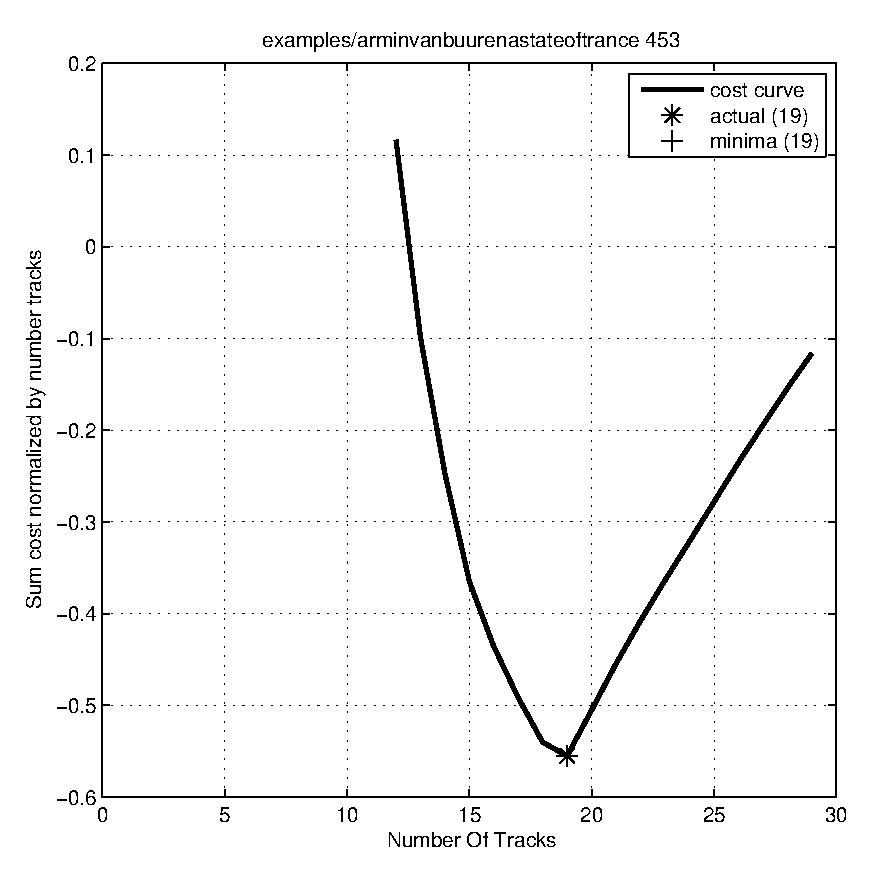
\includegraphics[width=0.5\textwidth]{images/trackestimate}
	\caption{Number of tracks estimated correctly a show in the GitHub training set after a genetics algorithm was executed to select a robust set of algorithm parameters.}
	\label{fig:github_trackestimation}
\end{figure}

\begin{figure}
	\centering
	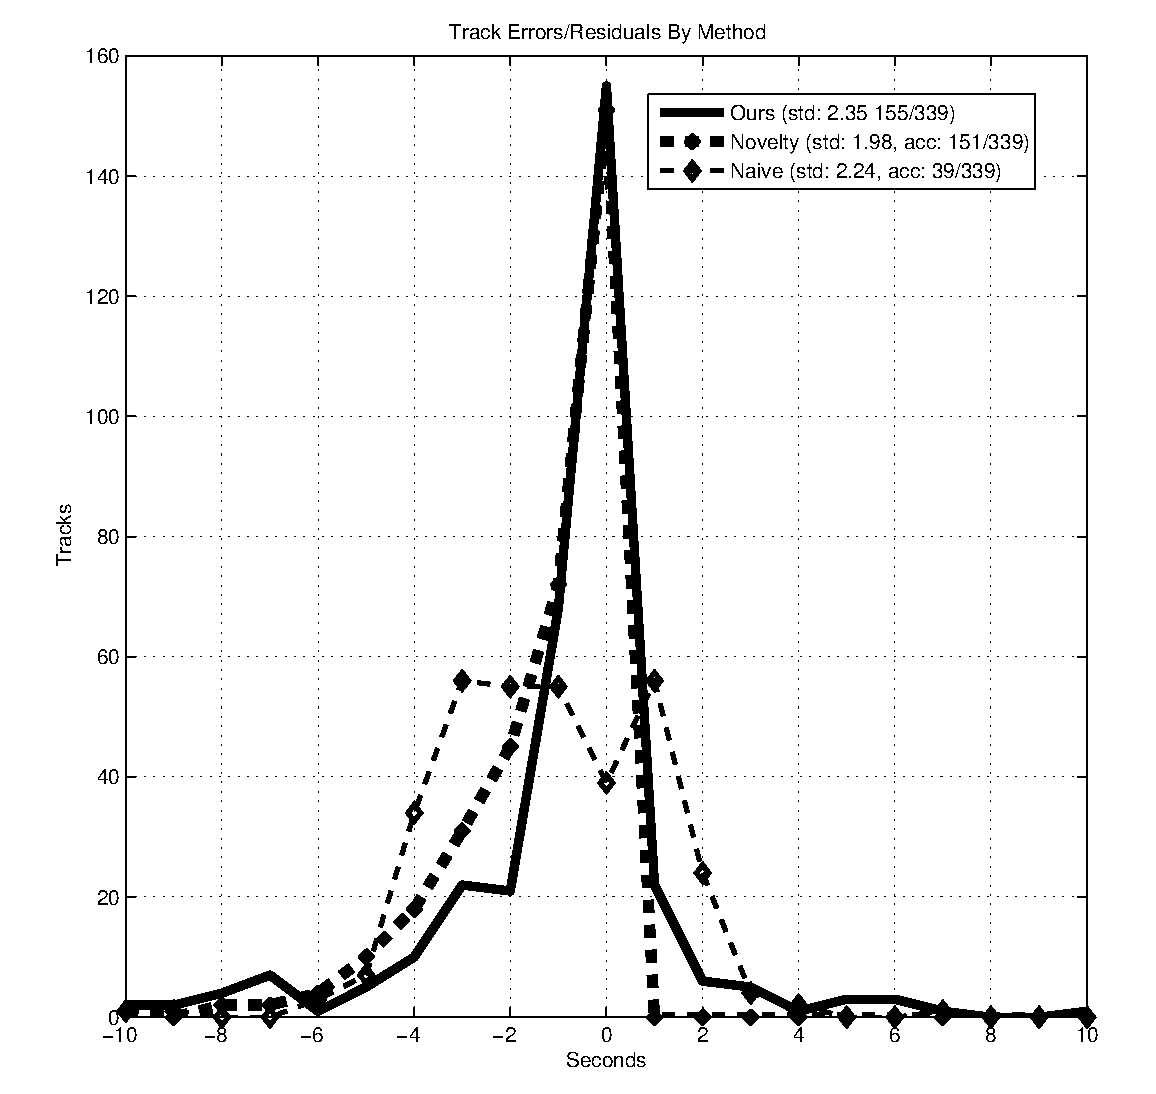
\includegraphics[width=0.5\textwidth]{images/trackshift}
	\caption{Track estimation error on our method as described in Section \ref{sec:trackcount}, Foote's novelty function and Naive guessing. }
	\label{fig:track_shift}
\end{figure}

\subsubsection{Comparison of Methods}

It is useful to compare our algorithm for reconstructing track boundaries with Foote's novelty peak finding method in a general sense. The drawback of Foote's method is that it is problematic to find a fixed number of novelty peaks. It is clearly adaptable to find a \textit{maximum} number of peaks but this does not help because it already has the interesting feature that it apparently rarely overestimates the number of tracks, it almost always underestimates.

We will henceforth transform the problem into one of binary classification subject to a variable threshold. When a predicted boundary is within a threshold time horizon $\tilde t$ of an actual boundary, it will be called a true positive. Otherwise, a true negative. We can borrow machine learning evaluators for binary classification problems; precision, recall and $F_1$ score.

Let

\[
F_1 = 2\frac{P \cdot R}{P+R}
\] be the harmonic mean of precision 
\[
P = \frac{|TP|}{|P|}
\]
 and recall (true positive rate)
\[
R=\frac{|TP|}{|A|}
\] subject to threshold time horizon $\tilde t$. Note $|P|$ denotes the number of predicted tracks tracks and $|A|$ the number of actual tracks in a given show.

\subsubsection{Results}

See Figure~\ref{fig:fscores_breakdown} for a break down of $F_1$ scores for each data set and Figure~\ref{fig:fscores_best} for the overall $F_1$ scores for the entire corpus, for all time thresholds. Note that guessing refers to placing tracks every $377$ seconds until no more can be placed. What is clear is that adding the radius enhancement to Foote's method significantly improves its performance and it slightly out-performs our algorithm when we estimate the number of tracks apart from on the \texttt{lindmik} dataset. 

Plotz \citep{plotz2006automatic} achieved a true positive rate of 81\% within $10$ second boundaries from ground truth for a similar task. Considering the standard deviation of human disagreement on annotations for dance music can be over $9$ seconds (see Section~\ref{human_acc}), this seems unobtainable with the corpus we have. Our overall true positive average is 63\% at the $10$ seconds threshold. For \texttt{tatw} we achieve 72.2\% which may be more like the corpora Plotz worked with.

When the number of tracks is known a priori, we significantly out-perform Foote's method. And there is no obvious way to modify Foote's method to select the correct number of tracks even if it is known a priori. 

It should be noted that our method of track estimation may be not be optimal. We only trained the evolutionary algorithm on $6$ shows on the \textit{GitHub training set} and estimated them all correctly. This meant the parameters found could possibly have been better. Increasing the size of the training set would address this issue. 

\section{Conclusion}\label{conclusions}

We believe our algorithm would be useful for segmenting DJ-mixed audio streams in batch mode. It would be excellent if \textit{SoundCloud}\footnote{\url{http://www.soundcloud.com}} for example started to do something similar. \textit{SoundCloud} is an on-line music service with many electronic dance music radio shows with the track listing in text. This method would allow them to reliably segment the shows, and they could display an interactive segmentation in the music player. 

The new cost matrices in combination improve robustness significantly over a summation cost matrix alone. They are also partly immunised against dissimilar regions within tracks which was a weakness in \citep{scarfe2013long}. One problem that we are aware of is the rare instances when there are head or tail segments to a track that seem independent from the rest of the track. When these are small they usually get absorbed without any problems but they can cause misplacements.

We are able to operate in the scenario when the number of tracks is not known a priori and perform comparably with our \textit{enhanced} version of Foote's \citep{foote2003media} method for both segmentation and estimation of how many tracks exist in a recording. On the \texttt{lindmik} dataset, we out-perform the enhanced Foote method. Our method comes into its own however in the scenario when the number of tracks is known a priori. We significantly out perform Foote's method for this and there is no constructive way to adapt Foote's method to find a fixed number of tracks. 

Further work includes the plan to write an on-line version of the algorithm in the future which will operate on a sliding lagged window of audio where the number of tracks could be estimated and the algorithm executed on the window. We would also like to implement a regularised version of Radu's time dependent agglomerative (hierarchical) clustering algorithm \citep{radu} to see if it is suitable for this task. 

One of the interesting properties of the algorithm presented here is that is it does not directly consider inter-segment dissimilarity. The costs are computed only from intra-segment similarity. Therefore; there is only an implied notion of dissimilarity between segments. An interesting direction would be reformulating the algorithm to consider transitional \textit{switching} and \textit{sticking} costs through a state graph where the number of switches was fixed a priori. This would be a somewhat similar direction to \citep{goodwin2003audio,goodwin2004dynamic} apart from the likelihood that fixing the number of segments a priori if they were known would likely improve the accuracy of the annotations as we have reported for this configuration.

\begin{table*}[h]
	\centering
	
	\scalebox{0.75}{
	\begin{tabular}{llll@{}llllllllllllllllll@{}}
			& \begin{sideways} \textsc{Domain} \end{sideways}	& \begin{sideways} \textsc{Notation} \end{sideways} & \begin{sideways}\textsc{Mean All}\end{sideways} & \begin{sideways}\textsc{Mean Contig}\end{sideways} & \begin{sideways}\textsc{Mean Evolution}\end{sideways} & \begin{sideways}\textsc{Mean Sum}\end{sideways} & \begin{sideways}\textsc{Mean Symmetry}\end{sideways} & \begin{sideways}\textsc{Median All}\end{sideways} & \begin{sideways}\textsc{Median Contig}\end{sideways} & \begin{sideways}\textsc{Median Evolution}\end{sideways} & \begin{sideways}\textsc{Median Sum}\end{sideways} & \begin{sideways}\textsc{Median Symmetry}\end{sideways} & \begin{sideways}\textsc{Track Estimation}\end{sideways} \\
		\toprule
		\textsc{Experiment Number}          &                   &            & 1     & 2    & 3    & 4    & 5    & 6    & 7    & 8    & 9    & 10   & 11   &  \\ \toprule
		\texttt{Seconds Per Tile (S) }      & $3,\ldots,50$     & $M$        & 3     & 3    & 6    & 5    & 8    & 3    & 7    & 3    & 5    & 9    & 38   &  \\
		\texttt{Min. Track Length (S) }     & $80,\ldots,180$   & $w$        & 167   & 146  & 108  & 165  & 140  & 88   & 98   & 173  & 94   & 85   & 155  &  \\
		\texttt{Max. Track Length (S) }     & $600,\ldots,900$  & $W$        & 691   & 879  & 897  & 894  & 811  & 631  & 801  & 889  & 642  & 635  & 619  &  \\
		\texttt{Bandwidth (Hz)      }       & $1,\ldots,15$     & $b$        & 1     & 2    & 2    & 2    & 3    & 2    & 4    & 4    & 2    & 5    & 3    &  \\
		\texttt{Low Pass Filter (Hz) }      & $800,\ldots,1950$ & $l$        & 1039~ & 1912 & 1893 & 1387 & 874  & 888  & 1065 & 1206 & 1880 & 1005 & 1019 &  \\
		\texttt{High Pass Filter (Hz)}      & $50,\ldots,500$   & $h$        & 62    & 73   & 81   & 69   & 54   & 55   & 54   & 70   & 75   & 51   & 201  &  \\
		\texttt{Solution Shift (S) }        & $-3,\ldots,5$     & $ \varXi $ & -1    & 5    & -3   & -2   & 2    & -4   & -2   & -2   & -2   & -1   & 5    &  \\
		\texttt{Cosine Normalization }      & $[0.4,1.4]$       & $\hat c$   & 1.17  & 0.77 & 0.92 & 1.19 & 1.36 & 0.88 & 0.71 & 0.73 & 1.15 & 1.14 & 0.98 &  \\ \midrule
		\texttt{Sum Contribution  }         & $[0,1]$           &            & 0.99  &      &      & 0.81 &      & 0.77 &      &      & 0.63 &      & 0.55 &  \\
		\texttt{Sum Normalization }         & $[0,1]$           &            & 1.36  &      &      & 0.73 &      & 1.11 &      &      & 0.47 &      & 0.71 &  \\
		\texttt{Sum Incentive      }        & $[0,1]$           &            & 0.68  &      &      & 0.52 &      & 0.23 &      &      & 0.30 &      & 0.05 &  \\ \midrule
		\texttt{Gaussian Contribution  }    & $[0,1]$           &            & 0.52  & 0.08 & 0.69 & 0.17 & 0.29 & 0.63 & 0.11 & 0.51 & 0.08 & 0.02 & 0.15 &  \\
		\texttt{Gaussian Incentive}         & $[0,1]$           &            & 0.85  & 0.82 & 0.43 & 0.47 & 0.56 & 0.10 & 0.14 & 0.40 & 0.85 & 0.54 & 0.53 &  \\
		\texttt{Gaussian Width  }           & $1,\ldots,4$      & $\varpi$   & 1     & 1    & 1    & 4    & 1    & 1    & 2    & 1    & 1    & 2    & 4    &  \\ \midrule
		\texttt{Evolution Contribution}     & $[0,1]$           &            & 0.05  &      & 0.63 &      &      & 0.49 &      & 0.35 &      &      & 0.48 &  \\
		\texttt{Evolution Incentive}        & $[0,1]$           &            & 0.53  &      & 0.60 &      &      & 0.15 &      & 0.66 &      &      & 0.71 &  \\
		\texttt{Evolution Normalization}    & $[0.1,3]$         &            & 1.30  &      & 0.08 &      &      & 1.10 &      & 0.06 &      &      & 1.79 &  \\
		\texttt{Evolution Diff. Order}      & $1,\ldots,50$     &            & 45    &      & 1    &      &      & 7    &      & 40   &      &      & 16   &  \\ \midrule
		\texttt{Contig Past Contribution}   & $[0,1]$           &            & 0.50  & 0.10 &      &      &      & 0.62 & 0.69 &      &      &      & 0.27 &  \\
		\texttt{Contig Past Diff. Order}    & $1,\ldots,50$     &            & 13    & 44   &      &      &      & 41   & 46   &      &      &      & 30   &  \\
		\texttt{Contig Past Incentive}      & $[0,1]$           &            & 0.50  & 0.24 &      &      &      & 0.95 & 0.53 &      &      &      & 0.98 &  \\
		\texttt{Contig Normalization}       & $[0.1,3]$         &            & 0.74  & 0.26 &      &      &      & 1.60 & 0.33 &      &      &      & 1.91 &  \\
		\texttt{Contig Future Contribution} & $[0,1]$           &            & 0.59  & 0.81 &      &      &      & 0.54 & 0.27 &      &      &      & 0.95 &  \\
		\texttt{Contig Future Diff. Order}  & $1,\ldots,50$     &            & 35    & 3    &      &      &      & 30   & 21   &      &      &      & 45   &  \\
		\texttt{Contig Future Incentive}    & $[0,1]$           &            & 0.08  & 0.24 &      &      &      & 0.60 & 0.89 &      &      &      & 0.96 &  \\ \midrule
		\texttt{Symmetry Contribution}      & $[0,1]$           &            & 0.18  &      &      &      & 0.66 & 0.11 &      &      &      & 0.98 & 0.19 &  \\
		\texttt{Symmetry Incentive}         & $[0,1]$           &            & 0.16  &      &      &      & 0.78 & 0.24 &      &      &      & 0.45 & 0.26 &  \\
		\texttt{Symmetry Normalization}     & $[0.1,3]$         &            & 0.73  &      &      &      & 0.77 & 0.72 &      &      &      & 0.55 & 1.09 &  \\ \bottomrule
		                                    &                   &
	\end{tabular}
}
	\caption{Results for stochastic optimization (evolutionary algorithm) search of parameter space. Note that the search space $T$ was limited to a minimum of $3$ seconds to save computation time.  }
	\label{tab:parameters}
\end{table*}


\section{Acknowledgements}\label{sec:acknowledgements}

We would like to thank Mikael Lindgren and Denis Goncharov from cuenation\footnote{\url{http://www.cuenation.com}} for their help explaining how they make cue-sheets and for providing the data set to test the algorithm on.

\section{Materials}\label{sec:materials}

All the code presented in this paper with the training set is available on GitHub\footnote{\url{github.com/ecsplendid/DanceMusicSegmentation}}. The corpus ($\approx150$GB) we received from Denis Goncharov and Mikael Lindgren will be made available on request (it is in a cloud storage account).


\bibliographystyle{ieeetr}
\bibliography{bib/references,bib/refs}

\end{document}
